% Options for packages loaded elsewhere
\PassOptionsToPackage{unicode}{hyperref}
\PassOptionsToPackage{hyphens}{url}
%
\documentclass[
]{article}
\usepackage{amsmath,amssymb}
\usepackage{iftex}
\ifPDFTeX
  \usepackage[T1]{fontenc}
  \usepackage[utf8]{inputenc}
  \usepackage{textcomp} % provide euro and other symbols
\else % if luatex or xetex
  \usepackage{unicode-math} % this also loads fontspec
  \defaultfontfeatures{Scale=MatchLowercase}
  \defaultfontfeatures[\rmfamily]{Ligatures=TeX,Scale=1}
\fi
\usepackage{lmodern}
\ifPDFTeX\else
  % xetex/luatex font selection
\fi
% Use upquote if available, for straight quotes in verbatim environments
\IfFileExists{upquote.sty}{\usepackage{upquote}}{}
\IfFileExists{microtype.sty}{% use microtype if available
  \usepackage[]{microtype}
  \UseMicrotypeSet[protrusion]{basicmath} % disable protrusion for tt fonts
}{}
\makeatletter
\@ifundefined{KOMAClassName}{% if non-KOMA class
  \IfFileExists{parskip.sty}{%
    \usepackage{parskip}
  }{% else
    \setlength{\parindent}{0pt}
    \setlength{\parskip}{6pt plus 2pt minus 1pt}}
}{% if KOMA class
  \KOMAoptions{parskip=half}}
\makeatother
\usepackage{xcolor}
\usepackage[margin=1in]{geometry}
\usepackage{color}
\usepackage{fancyvrb}
\newcommand{\VerbBar}{|}
\newcommand{\VERB}{\Verb[commandchars=\\\{\}]}
\DefineVerbatimEnvironment{Highlighting}{Verbatim}{commandchars=\\\{\}}
% Add ',fontsize=\small' for more characters per line
\usepackage{framed}
\definecolor{shadecolor}{RGB}{248,248,248}
\newenvironment{Shaded}{\begin{snugshade}}{\end{snugshade}}
\newcommand{\AlertTok}[1]{\textcolor[rgb]{0.94,0.16,0.16}{#1}}
\newcommand{\AnnotationTok}[1]{\textcolor[rgb]{0.56,0.35,0.01}{\textbf{\textit{#1}}}}
\newcommand{\AttributeTok}[1]{\textcolor[rgb]{0.13,0.29,0.53}{#1}}
\newcommand{\BaseNTok}[1]{\textcolor[rgb]{0.00,0.00,0.81}{#1}}
\newcommand{\BuiltInTok}[1]{#1}
\newcommand{\CharTok}[1]{\textcolor[rgb]{0.31,0.60,0.02}{#1}}
\newcommand{\CommentTok}[1]{\textcolor[rgb]{0.56,0.35,0.01}{\textit{#1}}}
\newcommand{\CommentVarTok}[1]{\textcolor[rgb]{0.56,0.35,0.01}{\textbf{\textit{#1}}}}
\newcommand{\ConstantTok}[1]{\textcolor[rgb]{0.56,0.35,0.01}{#1}}
\newcommand{\ControlFlowTok}[1]{\textcolor[rgb]{0.13,0.29,0.53}{\textbf{#1}}}
\newcommand{\DataTypeTok}[1]{\textcolor[rgb]{0.13,0.29,0.53}{#1}}
\newcommand{\DecValTok}[1]{\textcolor[rgb]{0.00,0.00,0.81}{#1}}
\newcommand{\DocumentationTok}[1]{\textcolor[rgb]{0.56,0.35,0.01}{\textbf{\textit{#1}}}}
\newcommand{\ErrorTok}[1]{\textcolor[rgb]{0.64,0.00,0.00}{\textbf{#1}}}
\newcommand{\ExtensionTok}[1]{#1}
\newcommand{\FloatTok}[1]{\textcolor[rgb]{0.00,0.00,0.81}{#1}}
\newcommand{\FunctionTok}[1]{\textcolor[rgb]{0.13,0.29,0.53}{\textbf{#1}}}
\newcommand{\ImportTok}[1]{#1}
\newcommand{\InformationTok}[1]{\textcolor[rgb]{0.56,0.35,0.01}{\textbf{\textit{#1}}}}
\newcommand{\KeywordTok}[1]{\textcolor[rgb]{0.13,0.29,0.53}{\textbf{#1}}}
\newcommand{\NormalTok}[1]{#1}
\newcommand{\OperatorTok}[1]{\textcolor[rgb]{0.81,0.36,0.00}{\textbf{#1}}}
\newcommand{\OtherTok}[1]{\textcolor[rgb]{0.56,0.35,0.01}{#1}}
\newcommand{\PreprocessorTok}[1]{\textcolor[rgb]{0.56,0.35,0.01}{\textit{#1}}}
\newcommand{\RegionMarkerTok}[1]{#1}
\newcommand{\SpecialCharTok}[1]{\textcolor[rgb]{0.81,0.36,0.00}{\textbf{#1}}}
\newcommand{\SpecialStringTok}[1]{\textcolor[rgb]{0.31,0.60,0.02}{#1}}
\newcommand{\StringTok}[1]{\textcolor[rgb]{0.31,0.60,0.02}{#1}}
\newcommand{\VariableTok}[1]{\textcolor[rgb]{0.00,0.00,0.00}{#1}}
\newcommand{\VerbatimStringTok}[1]{\textcolor[rgb]{0.31,0.60,0.02}{#1}}
\newcommand{\WarningTok}[1]{\textcolor[rgb]{0.56,0.35,0.01}{\textbf{\textit{#1}}}}
\usepackage{graphicx}
\makeatletter
\def\maxwidth{\ifdim\Gin@nat@width>\linewidth\linewidth\else\Gin@nat@width\fi}
\def\maxheight{\ifdim\Gin@nat@height>\textheight\textheight\else\Gin@nat@height\fi}
\makeatother
% Scale images if necessary, so that they will not overflow the page
% margins by default, and it is still possible to overwrite the defaults
% using explicit options in \includegraphics[width, height, ...]{}
\setkeys{Gin}{width=\maxwidth,height=\maxheight,keepaspectratio}
% Set default figure placement to htbp
\makeatletter
\def\fps@figure{htbp}
\makeatother
\setlength{\emergencystretch}{3em} % prevent overfull lines
\providecommand{\tightlist}{%
  \setlength{\itemsep}{0pt}\setlength{\parskip}{0pt}}
\setcounter{secnumdepth}{-\maxdimen} % remove section numbering
\usepackage{booktabs}
\usepackage{longtable}
\usepackage{array}
\usepackage{multirow}
\usepackage{wrapfig}
\usepackage{float}
\usepackage{colortbl}
\usepackage{pdflscape}
\usepackage{tabu}
\usepackage{threeparttable}
\usepackage{threeparttablex}
\usepackage[normalem]{ulem}
\usepackage{makecell}
\usepackage{xcolor}
\ifLuaTeX
  \usepackage{selnolig}  % disable illegal ligatures
\fi
\usepackage{bookmark}
\IfFileExists{xurl.sty}{\usepackage{xurl}}{} % add URL line breaks if available
\urlstyle{same}
\hypersetup{
  pdftitle={Introduction to linear mixed models},
  pdfauthor={Edwin Yánez},
  hidelinks,
  pdfcreator={LaTeX via pandoc}}

\title{Introduction to linear mixed models}
\author{Edwin Yánez}
\date{2025-04-22}

\begin{document}
\maketitle

{
\setcounter{tocdepth}{4}
\tableofcontents
}
\subsection{Purpose}\label{purpose}

This is a follow-along document reporting my engagement with Coding
Club's
\href{https://ourcodingclub.github.io/tutorials/mixed-models/index.html}{Introduction
to linear mixed models} tutorial. Not everything in the tutorial is
expected to be replicated here.

\subsection{1. What is mixed effects modelling and why does it
matter?}\label{what-is-mixed-effects-modelling-and-why-does-it-matter}

Ecological and biological data are often complex and messy. We can have
different grouping factors like populations, species, sites where we
collect the data, etc. Sample sizes might leave something to be desired
too, especially if we are trying to fit complicated models with many
parameters. On top of that, our data points might not be truly
independent. For instance, we might be using quadrats within our sites
to collect the data (and so there is structure to our data: quadrats are
nested within the sites).

This is why mixed models were developed, to deal with such messy data
and to allow us to use all our data, even when we have low sample sizes,
structured data and many covariates to fit. Oh, and on top of all that,
mixed models allow us to save degrees of freedom compared to running
standard linear models! Sounds good, doesn't it?

We will cover only linear mixed models here, but if you are trying to
``extend'' your linear model, fear not: there are generalised linear
mixed effects models out there, too.

\subsection{2. Explore the data}\label{explore-the-data}

We are going to focus on a fictional study system, dragons, so that we
don't have to get too distracted with the specifics of this example.
Imagine that we decided to train dragons and so we went out into the
mountains and collected data on dragon intelligence (testScore) as a
prerequisite. We sampled individuals with a range of body lengths across
three sites in eight different mountain ranges. Start by loading the
data and having a look at them.

\begin{Shaded}
\begin{Highlighting}[]
\FunctionTok{load}\NormalTok{(}\StringTok{\textquotesingle{}dragons.RData\textquotesingle{}}\NormalTok{)}
\NormalTok{dragons }\OtherTok{\textless{}{-}} \FunctionTok{as\_tibble}\NormalTok{(dragons)}
\NormalTok{dragons}
\end{Highlighting}
\end{Shaded}

\begin{verbatim}
## # A tibble: 480 x 5
##    testScore bodyLength mountainRange X     site 
##        <dbl>      <dbl> <fct>         <lgl> <fct>
##  1     16.1        166. Bavarian      NA    a    
##  2     33.9        168. Bavarian      NA    a    
##  3      6.04       166. Bavarian      NA    a    
##  4     18.8        168. Bavarian      NA    a    
##  5     33.9        170. Bavarian      NA    a    
##  6     47.0        169. Bavarian      NA    a    
##  7      2.56       170. Bavarian      NA    a    
##  8      3.88       164. Bavarian      NA    a    
##  9      3.60       168. Bavarian      NA    a    
## 10      7.36       180. Bavarian      NA    a    
## # i 470 more rows
\end{verbatim}

Let's say we want to know how the body length of the dragons affects
their test scores.

You don't need to worry about the distribution of your explanatory
variables. Have a look at the distribution of the response variable:

\begin{Shaded}
\begin{Highlighting}[]
\FunctionTok{hist}\NormalTok{(dragons}\SpecialCharTok{$}\NormalTok{testScore)  }\CommentTok{\# seems close to a normal distribution {-} good!}
\end{Highlighting}
\end{Shaded}

\begin{center}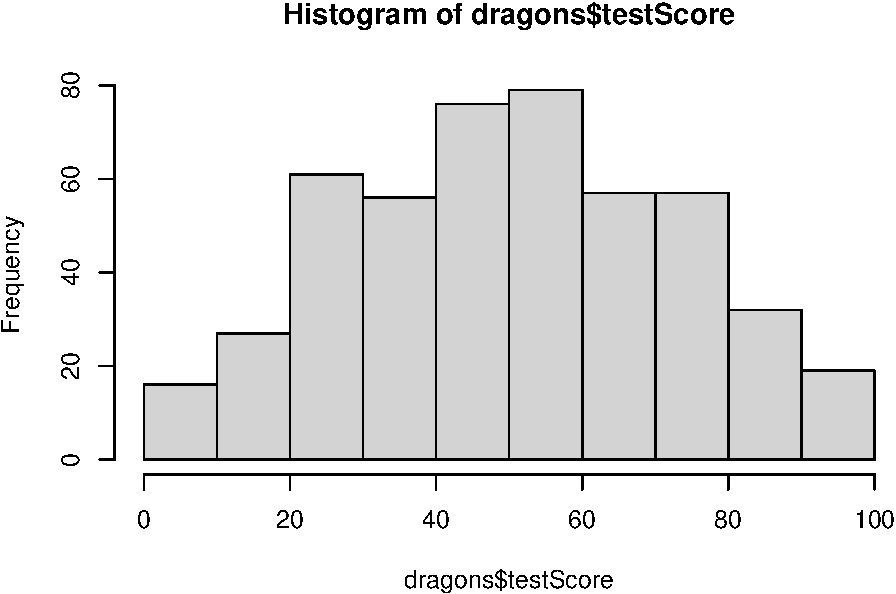
\includegraphics{Introduction-to-linear-mixed-models_files/figure-latex/unnamed-chunk-2-1} \end{center}

It is good practice to standardise your explanatory variables before
proceeding so that they have a mean of zero (``centering'') and standard
deviation of one (``scaling''). It ensures that the estimated
coefficients are all on the same scale, making it easier to compare
effect sizes. You can use scale() to do that:

\begin{Shaded}
\begin{Highlighting}[]
\NormalTok{dragons }\OtherTok{\textless{}{-}}\NormalTok{ dragons }\SpecialCharTok{\%\textgreater{}\%} 
  \FunctionTok{mutate}\NormalTok{(}
    \AttributeTok{bodyLength2 =} \FunctionTok{as.vector}\NormalTok{(}\FunctionTok{scale}\NormalTok{(bodyLength))}
\NormalTok{  )}
\end{Highlighting}
\end{Shaded}

\subsection{3. Fit all data in one
analysis}\label{fit-all-data-in-one-analysis}

One way to analyse this data would be to fit a linear model to all our
data, ignoring the sites and the mountain ranges for now.

Fit the model with testScore as the response and bodyLength2 as the
predictor and have a look at the output:

\begin{Shaded}
\begin{Highlighting}[]
\NormalTok{basic\_lm }\OtherTok{\textless{}{-}} \FunctionTok{lm}\NormalTok{(testScore }\SpecialCharTok{\textasciitilde{}}\NormalTok{ bodyLength2, }\AttributeTok{data =}\NormalTok{ dragons)}
\FunctionTok{summary}\NormalTok{(basic\_lm)}
\end{Highlighting}
\end{Shaded}

\begin{verbatim}
## 
## Call:
## lm(formula = testScore ~ bodyLength2, data = dragons)
## 
## Residuals:
##     Min      1Q  Median      3Q     Max 
## -56.962 -16.411  -0.783  15.193  55.200 
## 
## Coefficients:
##             Estimate Std. Error t value Pr(>|t|)    
## (Intercept)  50.3860     0.9676  52.072   <2e-16 ***
## bodyLength2   8.9956     0.9686   9.287   <2e-16 ***
## ---
## Signif. codes:  0 '***' 0.001 '**' 0.01 '*' 0.05 '.' 0.1 ' ' 1
## 
## Residual standard error: 21.2 on 478 degrees of freedom
## Multiple R-squared:  0.1529, Adjusted R-squared:  0.1511 
## F-statistic: 86.25 on 1 and 478 DF,  p-value: < 2.2e-16
\end{verbatim}

Let's plot the data with ggplot2.

\begin{Shaded}
\begin{Highlighting}[]
\NormalTok{prelim\_plot }\OtherTok{\textless{}{-}}\NormalTok{ dragons }\SpecialCharTok{\%\textgreater{}\%} 
  \FunctionTok{ggplot}\NormalTok{(}\FunctionTok{aes}\NormalTok{(}\AttributeTok{x =}\NormalTok{ bodyLength, }\AttributeTok{y =}\NormalTok{ testScore))}\SpecialCharTok{+}
  \FunctionTok{geom\_point}\NormalTok{()}\SpecialCharTok{+}
  \FunctionTok{geom\_smooth}\NormalTok{(}\AttributeTok{method =} \StringTok{\textquotesingle{}lm\textquotesingle{}}\NormalTok{)}
\NormalTok{prelim\_plot}
\end{Highlighting}
\end{Shaded}

\begin{verbatim}
## `geom_smooth()` using formula = 'y ~ x'
\end{verbatim}

\begin{center}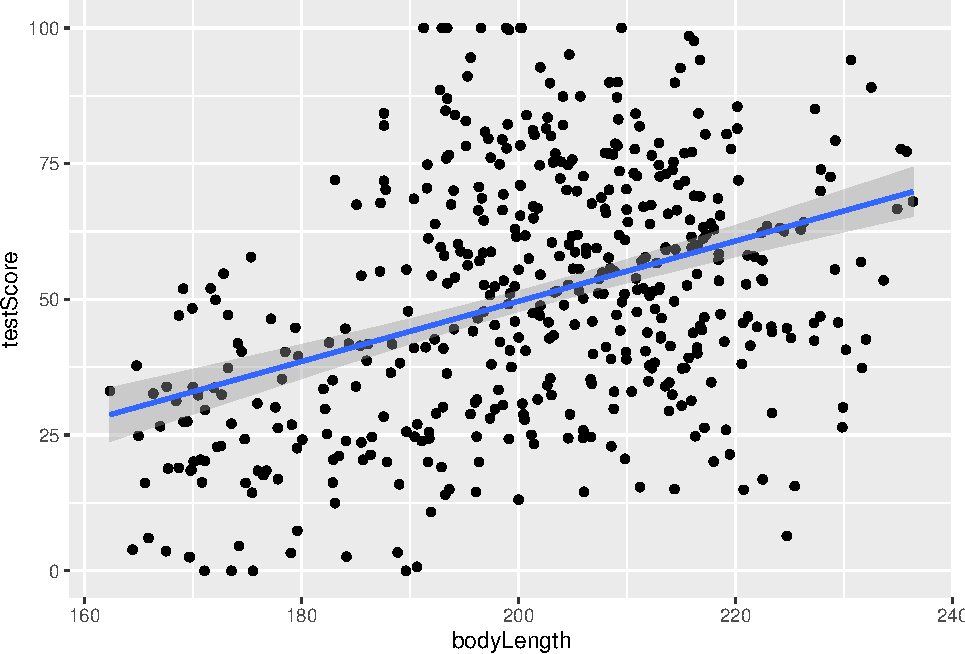
\includegraphics{Introduction-to-linear-mixed-models_files/figure-latex/unnamed-chunk-5-1} \end{center}

Okay, so both from the linear model and from the plot, it seems like
bigger dragons do better in our intelligence test. That seems a bit odd:
size shouldn't really affect the test scores.

But\ldots{} are the assumptions met?

Plot the residuals: the red line should be nearly flat, like the dashed
grey line:

\begin{Shaded}
\begin{Highlighting}[]
\FunctionTok{plot}\NormalTok{(basic\_lm, }\AttributeTok{which =} \DecValTok{1}\NormalTok{)}
\end{Highlighting}
\end{Shaded}

\begin{center}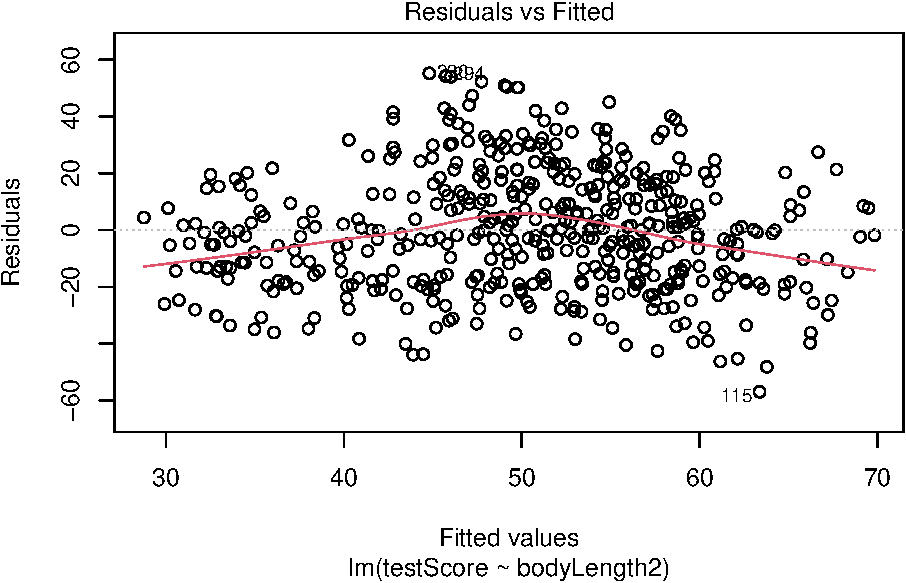
\includegraphics{Introduction-to-linear-mixed-models_files/figure-latex/unnamed-chunk-6-1} \end{center}

\begin{Shaded}
\begin{Highlighting}[]
\CommentTok{\# not perfect but since this is a fictional example we will go with it.}
\CommentTok{\# For real data: the bigger the sample size, the less of a trend one should expect to see.}
\end{Highlighting}
\end{Shaded}

Have a quick look at the qqplot too: points should ideally fall onto the
diagonal dashed line:

\begin{Shaded}
\begin{Highlighting}[]
\FunctionTok{plot}\NormalTok{(basic\_lm, }\AttributeTok{which =} \DecValTok{2}\NormalTok{)   }\CommentTok{\# a bit off at the extremes, but that\textquotesingle{}s often the case; again doesn\textquotesingle{}t look too bad}
\end{Highlighting}
\end{Shaded}

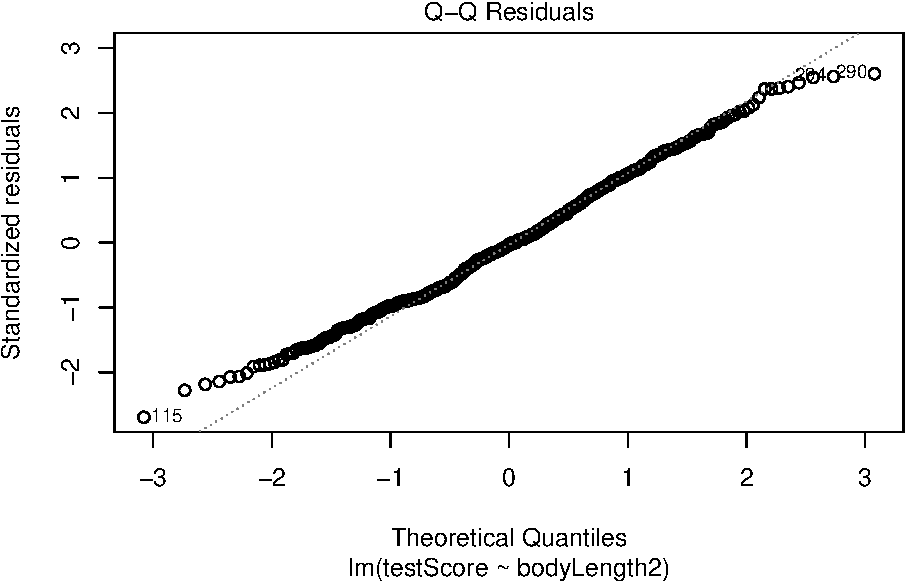
\includegraphics{Introduction-to-linear-mixed-models_files/figure-latex/unnamed-chunk-7-1.pdf}

However, what about observation independence? Are our data independent?

We collected multiple samples from eight mountain ranges. It's perfectly
plausible that the data from within each mountain range are more similar
to each other than the data from different mountain ranges: they are
correlated.

Have a look at the data to see if above is true:

\begin{Shaded}
\begin{Highlighting}[]
\FunctionTok{boxplot}\NormalTok{(testScore }\SpecialCharTok{\textasciitilde{}}\NormalTok{ mountainRange, }\AttributeTok{data =}\NormalTok{ dragons)   }\CommentTok{\# certainly looks like something is going on here}
\end{Highlighting}
\end{Shaded}

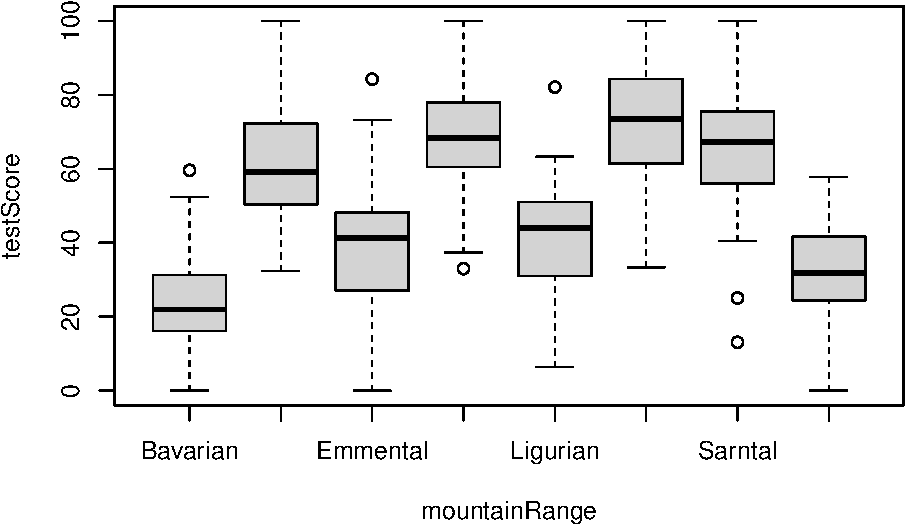
\includegraphics{Introduction-to-linear-mixed-models_files/figure-latex/unnamed-chunk-8-1.pdf}

\begin{Shaded}
\begin{Highlighting}[]
\NormalTok{p }\OtherTok{\textless{}{-}} \FunctionTok{ggplot}\NormalTok{(dragons, }\FunctionTok{aes}\NormalTok{(}\AttributeTok{x =}\NormalTok{ mountainRange, }\AttributeTok{y =}\NormalTok{ testScore))}\SpecialCharTok{+}
  \FunctionTok{geom\_boxplot}\NormalTok{()}\SpecialCharTok{+}
  \FunctionTok{theme\_classic}\NormalTok{()}
\NormalTok{p}
\end{Highlighting}
\end{Shaded}

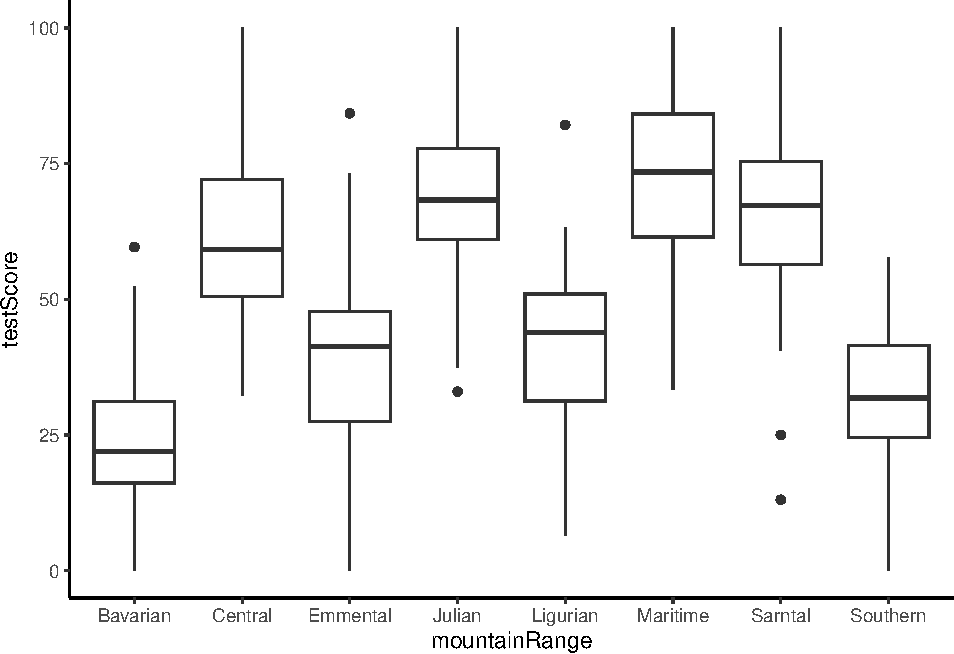
\includegraphics{Introduction-to-linear-mixed-models_files/figure-latex/unnamed-chunk-8-2.pdf}

We could also plot it and colour points by mountain range:

\begin{Shaded}
\begin{Highlighting}[]
\NormalTok{colour\_plot }\OtherTok{\textless{}{-}} \FunctionTok{ggplot}\NormalTok{(dragons, }\FunctionTok{aes}\NormalTok{(}\AttributeTok{x =}\NormalTok{ bodyLength, }\AttributeTok{y =}\NormalTok{ testScore, }\AttributeTok{colour =}\NormalTok{ mountainRange))}\SpecialCharTok{+}
  \FunctionTok{geom\_point}\NormalTok{(}\AttributeTok{size =} \DecValTok{2}\NormalTok{)}\SpecialCharTok{+}
  \FunctionTok{theme\_classic}\NormalTok{()}\SpecialCharTok{+}
  \FunctionTok{theme}\NormalTok{(}
    \AttributeTok{legend.position =} \StringTok{\textquotesingle{}\textquotesingle{}}
\NormalTok{  )}
\NormalTok{colour\_plot}
\end{Highlighting}
\end{Shaded}

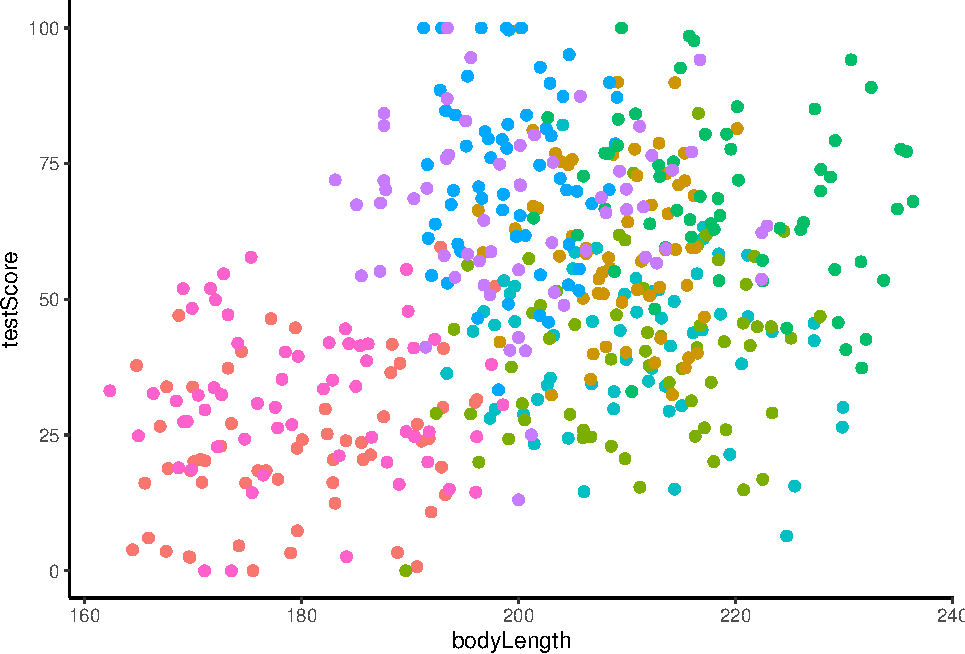
\includegraphics{Introduction-to-linear-mixed-models_files/figure-latex/unnamed-chunk-9-1.pdf}

From the above plots, it looks like our mountain ranges vary both in the
dragon body length AND in their test scores. This confirms that our
observations from within each of the ranges aren't independent. We can't
ignore that: as we're starting to see, it could lead to a completely
erroneous conclusion.

So what do we do?

\subsection{4. Run multiple analyses}\label{run-multiple-analyses}

We could run many separate analyses and fit a regression for each of the
mountain ranges.

Lets have a quick look at the data split by mountain range. We use the
facet\_wrap to do that:

\begin{Shaded}
\begin{Highlighting}[]
\NormalTok{split\_plot }\OtherTok{\textless{}{-}} \FunctionTok{ggplot}\NormalTok{(dragons, }\FunctionTok{aes}\NormalTok{(bodyLength, testScore))}\SpecialCharTok{+}
  \FunctionTok{geom\_point}\NormalTok{()}\SpecialCharTok{+}
  \FunctionTok{facet\_wrap}\NormalTok{(}\SpecialCharTok{\textasciitilde{}}\NormalTok{ mountainRange)}\SpecialCharTok{+}   \CommentTok{\# Create a facet for each mountain range}
  \FunctionTok{xlab}\NormalTok{(}\StringTok{\textquotesingle{}length\textquotesingle{}}\NormalTok{)}\SpecialCharTok{+}
  \FunctionTok{ylab}\NormalTok{(}\StringTok{\textquotesingle{}test score\textquotesingle{}}\NormalTok{)}
\NormalTok{split\_plot}
\end{Highlighting}
\end{Shaded}

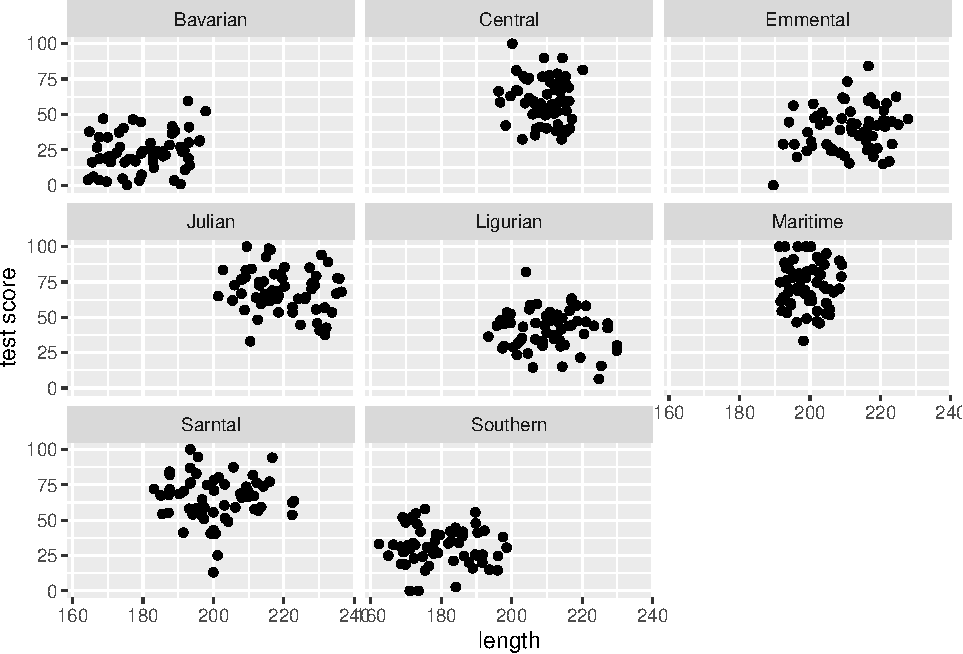
\includegraphics{Introduction-to-linear-mixed-models_files/figure-latex/unnamed-chunk-10-1.pdf}

That's eight analyses. Oh wait, we also have different sites in each
mountain range, which similarly to mountain ranges aren't
independent\ldots{} So we could run an analysis for each site in each
range separately.

To do the above, we would have to estimate a slope and intercept
parameter for each regression. That's two parameters, three sites and
eight mountain ranges, which means 48 parameter estimates (2 x 3 x 8 =
48)! Moreover, the sample size for each analysis would be only 20
(dragons per site).

This presents problems: not only are we hugely decreasing our sample
size, but we are also increasing chances of a Type I Error (where you
falsely reject the null hypothesis) by carrying out multiple
comparisons. Not ideal!

\subsection{5. Modify the current model}\label{modify-the-current-model}

We want to use all the data, but account for the data coming from
different mountain ranges (let's put sites on hold for a second to make
things simpler).

Add mountain range as a fixed effect to our \texttt{basic\_lm}

\begin{Shaded}
\begin{Highlighting}[]
\NormalTok{mountain\_lm }\OtherTok{\textless{}{-}} \FunctionTok{lm}\NormalTok{(testScore }\SpecialCharTok{\textasciitilde{}}\NormalTok{ bodyLength2 }\SpecialCharTok{+}\NormalTok{ mountainRange, }\AttributeTok{data =}\NormalTok{ dragons)}
\FunctionTok{summary}\NormalTok{(mountain\_lm)}
\end{Highlighting}
\end{Shaded}

\begin{verbatim}
## 
## Call:
## lm(formula = testScore ~ bodyLength2 + mountainRange, data = dragons)
## 
## Residuals:
##     Min      1Q  Median      3Q     Max 
## -52.263  -9.926   0.361   9.994  44.488 
## 
## Coefficients:
##                       Estimate Std. Error t value Pr(>|t|)    
## (Intercept)            23.3818     2.5792   9.065  < 2e-16 ***
## bodyLength2             0.2055     1.2927   0.159  0.87379    
## mountainRangeCentral   36.5828     3.5993  10.164  < 2e-16 ***
## mountainRangeEmmental  16.2092     3.6966   4.385 1.43e-05 ***
## mountainRangeJulian    45.1147     4.1901  10.767  < 2e-16 ***
## mountainRangeLigurian  17.7478     3.6736   4.831 1.84e-06 ***
## mountainRangeMaritime  49.8813     3.1392  15.890  < 2e-16 ***
## mountainRangeSarntal   41.9784     3.1972  13.130  < 2e-16 ***
## mountainRangeSouthern   8.5196     2.7313   3.119  0.00192 ** 
## ---
## Signif. codes:  0 '***' 0.001 '**' 0.01 '*' 0.05 '.' 0.1 ' ' 1
## 
## Residual standard error: 14.96 on 471 degrees of freedom
## Multiple R-squared:  0.5843, Adjusted R-squared:  0.5773 
## F-statistic: 82.76 on 8 and 471 DF,  p-value: < 2.2e-16
\end{verbatim}

Now body length is not significant. But let's think about what we are
doing here for a second. The above model is estimating the difference in
test scores between the mountain ranges - we can see all of them in the
model output returned by summary(). But we are not interested in
quantifying test scores for each specific mountain range: we just want
to know whether body length affects test scores and we want to simply
control for the variation coming from mountain ranges.

This is what we refer to as ``random factors'' and so we arrive at mixed
effects models. Ta-daa!

\subsection{6. Mixed effects models}\label{mixed-effects-models}

A mixed model is a good choice here: it will allow us to use all the
data we have (higher sample size) and account for the correlations
between data coming from the sites and mountain ranges. We will also
estimate fewer parameters and avoid problems with multiple comparisons
that we would encounter while using separate regressions.

We are going to work in lme4, so load the package (or use
install.packages if you don't have lme4 on your computer).

\subsubsection{Fixed and random effects}\label{fixed-and-random-effects}

Let's talk a little about the difference between fixed and random
effects first. It's important to not that this difference has little to
do with the variables themselves, and a lot to do with your research
question! In many cases, the same variable could be considered either a
random or a fixed effect (and sometimes even both at the same time!) so
always refer to your questions and hypotheses to construct your models
accordingly.

\begin{quote}
\textbf{Should my variables be fixed or random effects?} In broad terms,
fixed effects are variables that we expect will have an effect on the
dependent/response variable: they're what you call explanatory variables
in a standard linear regression. In our case, we are interested in
making conclusions about how dragon body length impacts the dragon's
test score. So body length is a fixed effect and test score is the
dependent variable.

On the other hand, random effects are usually grouping factors for which
we are trying to control. They are always categorical, as you can't
force R to treat a continuous variable as a random effect. A lot of the
time we are not specifically interested in their impact on the response
variable, but we know that they might be influencing the patterns we
see.

Additionally, the data for our random effect is just a sample of all the
possibilities: with unlimited time and funding we might have sampled
every mountain where dragons live, every school in the country, every
chocolate in the box), but we usually tend to generalise results to a
whole population based on representative sampling. We don't care about
estimating how much better pupils in school A have done compared to
pupils in school B, but we know that their respective teachers might be
a reason why their scores would be different, and we'd like to know how
much variation is attributable to this when we predict scores for pupils
in school Z.
\end{quote}

In our particular case, we are looking to control for the effects of
mountain range. We haven't sampled all the mountain ranges in the world
(we have eight) so our data are just a sample of all the existing
mountain ranges. We are not really interested in the effect of each
specific mountain range on the test score: we hope our model would also
be generalisable to dragons from other mountain ranges! However, we know
that the test scores from within the ranges might be correlated so we
want to control for that.

If we specifically chose eight particular mountain ranges a priori and
we were interested in those ranges and wanted to make predictions about
them, then mountain range would be fitted as a fixed effect.

\begin{quote}
\textbf{More about random effects} Note that the golden rule is that you
generally want your random effect to have \textbf{at least 5 levels}.
So, for instance, if we wanted to control for the effects of dragon's
sex on intelligence, we would fit sex (a two level factor: male or
female) \textbf{as a fixed, not random, effect.}

This is, put simply, because estimating variance on few data points is
very imprecise. Mathematically you could, but you wouldn't have a lot of
confidence in it. If you only have two or three levels, the model will
struggle to partition the variance - it will give you an output, but not
necessarily one you can trust.

Finally, keep in mind that the name random doesn't have much to do with
mathematical randomness. Yes, it's confusing. Just think about them as
the grouping variables for now. Strictly speaking it's all about making
our models representative of our questions \textbf{and getting better
estimates}. Hopefully, our next few examples will help you make sense of
how and why they're used.
\end{quote}

\textbf{In the end, the big questions are:} what are you trying to do?
What are you trying to make predictions about? What is just variation
(a.k.a ``noise'') that you need to control for?

\begin{quote}
Further reading for the keen:

\begin{itemize}
\tightlist
\item
  \href{https://dynamicecology.wordpress.com/2015/11/04/is-it-a-fixed-or-random-effect/}{Is
  it a fixed or random effect?} A useful way to think about fixed
  vs.~random effects is in terms of partitioning the variation and
  estimating random effects with partial pooling. The description here
  is the most accessible one I could find for now and you can find more
  opinions in the comments under the previous link too (search for
  pooling and shrinkage too if you are very keen).
\item
  \href{https://dynamicecology.wordpress.com/2015/02/05/how-many-terms-in-your-model-before-statistical-machismo/}{How
  many terms? On model complexity}
\item
  \href{https://dynamicecology.wordpress.com/2014/12/02/why-are-your-statistical-models-more-complex-these-days/}{More
  on model complexity}
\item
  Have a look at some of the fixed and random effects definitions
  gathered by Gelman in
  \href{https://sites.stat.columbia.edu/gelman/research/published/AOS259.pdf}{this
  paper} (you can also find them here if you can't access the paper).
\end{itemize}
\end{quote}

\subsubsection{Let's fit our first mixed
model}\label{lets-fit-our-first-mixed-model}

Alright! Still with me? We have a response variable, the test score and
we are attempting to explain part of the variation in test score through
fitting body length as a fixed effect. But the response variable has
some residual variation (i.e.~unexplained variation) associated with
mountain ranges. By using random effects, we are modeling that
unexplained variation through variance.

{[}Sidenote: If you are confused between variation and variance:
variation is a generic word, similar to dispersion or variability;
variance is a particular measure of variation; it quantifies the
dispersion, if you wish.{]}

Note that \textbf{our question changes slightly here}: while we still
want to know whether there is an association between dragon's body
length and the test score, we want to know if that association exists
after controlling for the variation in mountain ranges.

We will fit the random effect using the syntax (1\textbar variableName):

\begin{Shaded}
\begin{Highlighting}[]
\NormalTok{mixed.lmer }\OtherTok{\textless{}{-}} \FunctionTok{lmer}\NormalTok{(testScore }\SpecialCharTok{\textasciitilde{}}\NormalTok{ bodyLength2 }\SpecialCharTok{+}\NormalTok{ (}\DecValTok{1}\SpecialCharTok{|}\NormalTok{mountainRange), }\AttributeTok{data =}\NormalTok{ dragons)}
\FunctionTok{summary}\NormalTok{(mixed.lmer)}
\end{Highlighting}
\end{Shaded}

\begin{verbatim}
## Linear mixed model fit by REML ['lmerMod']
## Formula: testScore ~ bodyLength2 + (1 | mountainRange)
##    Data: dragons
## 
## REML criterion at convergence: 3985.6
## 
## Scaled residuals: 
##     Min      1Q  Median      3Q     Max 
## -3.4815 -0.6513  0.0066  0.6685  2.9583 
## 
## Random effects:
##  Groups        Name        Variance Std.Dev.
##  mountainRange (Intercept) 339.7    18.43   
##  Residual                  223.8    14.96   
## Number of obs: 480, groups:  mountainRange, 8
## 
## Fixed effects:
##             Estimate Std. Error t value
## (Intercept)  50.3860     6.5517   7.690
## bodyLength2   0.5377     1.2750   0.422
## 
## Correlation of Fixed Effects:
##             (Intr)
## bodyLength2 0.000
\end{verbatim}

Keep in mind that the random effect of the mountain range is meant to
capture all the influences of mountain ranges on dragon test scores -
whether we observed those influences explicitly or not, whether those
influences are big or small etc. It could be many, many teeny-tiny
influences that, when combined, affect the test scores and that's what
we are hoping to control for.

We can see the variance for mountainRange = 339.7. Mountain ranges are
clearly important: they explain a lot of variation. How do we know that?
We can take the variance for the mountainRange and divide it by the
total variance:

\begin{Shaded}
\begin{Highlighting}[]
\FloatTok{339.7}\SpecialCharTok{/}\NormalTok{(}\FloatTok{339.7} \SpecialCharTok{+} \FloatTok{223.8}\NormalTok{)  }\CommentTok{\# \textasciitilde{}60 \%}
\end{Highlighting}
\end{Shaded}

\begin{verbatim}
## [1] 0.6028394
\end{verbatim}

So the differences between mountain ranges explain \textasciitilde60\%
of the variance that's ``left over'' after the variance explained by our
fixed effects.

\begin{quote}
More reading on random effects Still confused about interpreting random
effects? These links have neat demonstrations and explanations:

\begin{itemize}
\tightlist
\item
  \href{https://www.r-bloggers.com/making-sense-of-random-effects/}{R-bloggers:
  Making sense of random effects}
\item
  \href{https://www.theanalysisfactor.com/understanding-random-effects-in-mixed-models/}{The
  Analysis Factor: Understanding random effects in mixed models}
\item
  \href{http://www.bodowinter.com/tutorial/bw_LME_tutorial.pdf}{Bodo
  Winter: A very basic tutorial for performing linear mixed effect
  analyses}
\end{itemize}
\end{quote}

As always, it's good practice to have a look at the plots to check our
assumptions:

\begin{Shaded}
\begin{Highlighting}[]
\FunctionTok{plot}\NormalTok{(mixed.lmer)   }\CommentTok{\# looks alright, no patterns evident}
\end{Highlighting}
\end{Shaded}

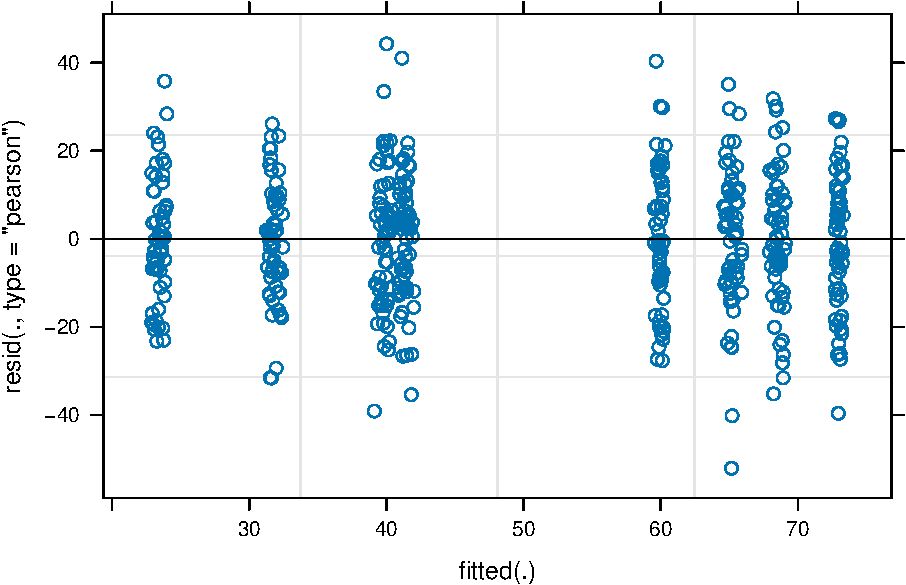
\includegraphics{Introduction-to-linear-mixed-models_files/figure-latex/unnamed-chunk-14-1.pdf}

and qqplot:

\begin{Shaded}
\begin{Highlighting}[]
\FunctionTok{qqnorm}\NormalTok{(}\FunctionTok{resid}\NormalTok{(mixed.lmer))}
\FunctionTok{qqline}\NormalTok{(}\FunctionTok{resid}\NormalTok{(mixed.lmer))   }\CommentTok{\# points fall nicely onto the line {-} good!}
\end{Highlighting}
\end{Shaded}

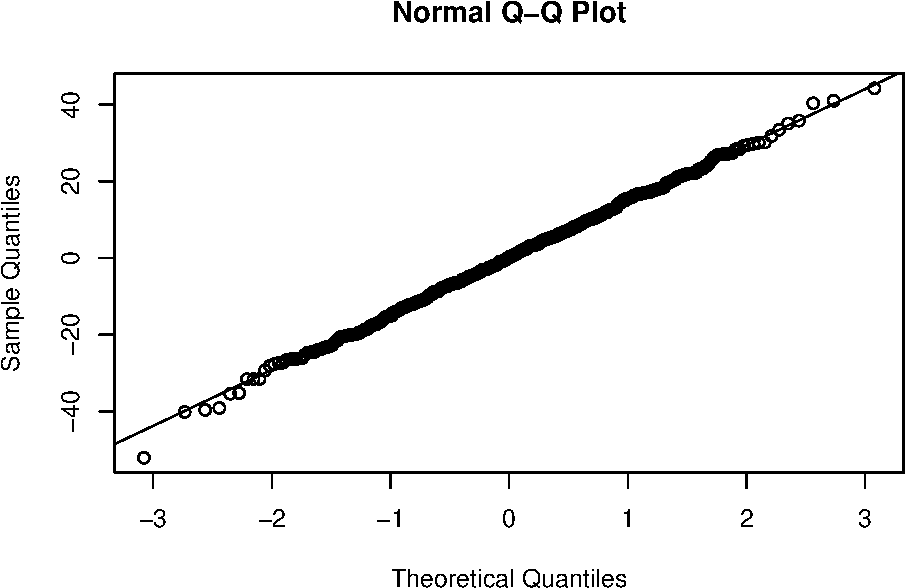
\includegraphics{Introduction-to-linear-mixed-models_files/figure-latex/unnamed-chunk-15-1.pdf}

\subsubsection{Types of random effects}\label{types-of-random-effects}

Before we go any further, let's review the syntax above and chat about
crossed and nested random effects. It's useful to get those clear in
your head.

\textbf{Reminder}: a factor is just any categorical independent
variable.

Above, we used \texttt{(1\textbar{}mountainRange)} to fit our random
effect. Whatever is on the right side of the \textbar{} operator is a
factor and referred to as a ``grouping factor'' for the term.

\textbf{Random effects (factors) can be crossed or nested} - it depends
on the relationship between the variables. Let's have a look.

\paragraph{Crossed random effects}\label{crossed-random-effects}

Be careful with the nomenclature. There are ``hierarchical linear
models'' (HLMs) or ``multilevel models'' out there, but while all HLMs
are mixed models, not all mixed models are hierarchical. That's because
you can have crossed (or partially crossed) random factors that do not
represent levels in a hierarchy.

Think for instance about our study where you monitor dragons (subject)
across different mountain ranges (context) and imagine that we collect
multiple observations per dragon by giving it the test multiple times
(and risking pseudoreplication - but more on that later). Since our
dragons can fly, it's easy to imagine that we might observe the same
dragon across different mountain ranges, but also that we might not see
all the dragons visiting all of the mountain ranges. Therefore, we can
potentially observe every dragon in every mountain range (crossed) or at
least observe some dragons across some of the mountain ranges (partially
crossed). We would then fit the identity of the dragon and mountain
range as (partially) crossed random effects.

Let's repeat with another example: an effect is (fully) crossed when all
the subjects have experienced all the levels of that effect. For
instance, if you had a fertilisation experiment on seedlings growing in
a seasonal forest and took repeated measurements over time (say 3 years)
in each season, you may want to have a crossed factor called season
(Summer1, Autumn1, Winter1, Spring1, Summer2, \ldots, Spring3), i.e.~a
factor for each season of each year. This grouping factor would account
for the fact that all plants in the experiment, regardless of the fixed
(treatment) effect (i.e.~fertilised or not), may have experienced a very
hot summer in the second year, or a very rainy spring in the third year,
and those conditions could cause interference in the expected patterns.
You don't even need to have associated climate data to account for it!
You just know that all observations from spring 3 may be more similar to
each other because they experienced the same environmental quirks rather
than because they're responding to your treatment.

If this sounds confusing, not to worry - lme4 handles partially and
fully crossed factors well. Now, let's look at nested random effects and
how to specify them.

\paragraph{Nested random effects}\label{nested-random-effects}

If you're not sure what nested random effects are, think of those
Russian nesting dolls. We've already hinted that we call these models
hierarchical: there's often an element of scale, or sampling
stratification in there.

Take our fertilisation experiment example again; let's say you have 50
seedlings in each bed, with 10 control and 10 experimental beds. That's
1000 seedlings altogether. And let's say you went out collecting once in
each season in each of the 3 years. On each plant, you measure the
length of 5 leaves. That's\ldots.(lots of maths)\ldots5 leaves x 50
plants x 20 beds x 4 seasons x 3 years\ldots.. 60 000 measurements!

But if you were to run the analysis using a simple linear regression,
eg. leafLength \textasciitilde{} treatment , you would be committing the
crime (!!) of pseudoreplication, or massively increasing your sampling
size by using non-independent data. With a sample size of 60,000 you
would almost certainly get a ``significant'' effect of treatment which
may have no ecological meaning at all. And it violates the assumption of
independance of observations that is central to linear regression.

This is where our nesting dolls come in; leaves within a plant and
plants within a bed may be more similar to each other (e.g.~for genetic
and environmental reasons, respectively). You could therefore add a
random effect structure that accounts for this nesting:

leafLength \textasciitilde{} treatment + (1\textbar Bed/Plant/Leaf)

This way, the model will account for non independence in the data: the
same leaves have been sampled repeatedly, multiple leaves were measured
on an individual, and plants are grouped into beds which may receive
different amounts of sun, etc.

What about the crossed effects we mentioned earlier? If all the leaves
have been measured in all seasons, then your model would become
something like:

\texttt{leafLength\ \textasciitilde{}\ treatment\ +\ (1\textbar{}Bed/Plant/Leaf)\ +\ (1\textbar{}Season)}

Phew!

\paragraph{Implicit vs.~explicit
nesting}\label{implicit-vs.-explicit-nesting}

To make things easier for yourself, code your data properly and
\textbf{avoid implicit nesting}.

To tackle this, let's look at another aspect of our study: we collected
the data on dragons not only across multiple mountain ranges, but also
across several sites within those mountain ranges. If you don't remember
have another look at the data:

\begin{Shaded}
\begin{Highlighting}[]
\NormalTok{dragons}
\end{Highlighting}
\end{Shaded}

\begin{verbatim}
## # A tibble: 480 x 6
##    testScore bodyLength mountainRange X     site  bodyLength2
##        <dbl>      <dbl> <fct>         <lgl> <fct>       <dbl>
##  1     16.1        166. Bavarian      NA    a           -2.21
##  2     33.9        168. Bavarian      NA    a           -2.08
##  3      6.04       166. Bavarian      NA    a           -2.19
##  4     18.8        168. Bavarian      NA    a           -2.07
##  5     33.9        170. Bavarian      NA    a           -1.93
##  6     47.0        169. Bavarian      NA    a           -2.01
##  7      2.56       170. Bavarian      NA    a           -1.96
##  8      3.88       164. Bavarian      NA    a           -2.28
##  9      3.60       168. Bavarian      NA    a           -2.09
## 10      7.36       180. Bavarian      NA    a           -1.34
## # i 470 more rows
\end{verbatim}

\begin{Shaded}
\begin{Highlighting}[]
\FunctionTok{str}\NormalTok{(dragons)}
\end{Highlighting}
\end{Shaded}

\begin{verbatim}
## tibble [480 x 6] (S3: tbl_df/tbl/data.frame)
##  $ testScore    : num [1:480] 16.15 33.89 6.04 18.84 33.86 ...
##  $ bodyLength   : num [1:480] 166 168 166 168 170 ...
##  $ mountainRange: Factor w/ 8 levels "Bavarian","Central",..: 1 1 1 1 1 1 1 1 1 1 ...
##  $ X            : logi [1:480] NA NA NA NA NA NA ...
##  $ site         : Factor w/ 3 levels "a","b","c": 1 1 1 1 1 1 1 1 1 1 ...
##  $ bodyLength2  : num [1:480] -2.21 -2.08 -2.19 -2.07 -1.93 ...
\end{verbatim}

Just like we did with the mountain ranges, we have to assume that data
collected within our sites might be correlated and so we should include
sites as an additional random effect in our model.

Our site variable is a three-level factor, with sites called a, b and
c.~The nesting of the site within the mountain range is implicit - our
sites are meaningless without being assigned to specific mountain
ranges, i.e.~there is nothing linking site b of the Bavarian mountain
range with site b of the Central mountain range. To avoid future
confusion we should create a new variable that is explicitly nested.
Let's call it sample:

\begin{Shaded}
\begin{Highlighting}[]
\CommentTok{\# Tidy version}
\NormalTok{dragons\_mine }\OtherTok{\textless{}{-}}\NormalTok{ dragons }\SpecialCharTok{\%\textgreater{}\%} 
  \FunctionTok{mutate}\NormalTok{(}
    \AttributeTok{sample =}\NormalTok{ mountainRange}\SpecialCharTok{:}\NormalTok{site}
\NormalTok{  )}

\CommentTok{\# Tutorial version}
\NormalTok{dragons }\OtherTok{\textless{}{-}} \FunctionTok{within}\NormalTok{(dragons, sample }\OtherTok{\textless{}{-}} \FunctionTok{factor}\NormalTok{(mountainRange}\SpecialCharTok{:}\NormalTok{site))}
\end{Highlighting}
\end{Shaded}

Now it's obvious that we have 24 samples (8 mountain ranges x 3 sites)
and not just 3: our sample is a 24-level factor and we should use that
instead of using site in our models: each site belongs to a specific
mountain range.

To sum up: for nested random effects, the factor appears ONLY within a
particular level of another factor (each site belongs to a specific
mountain range and only to that range); for crossed effects, a given
factor appears in more than one level of another factor (dragons
appearing within more than one mountain range). Or you can just remember
that if your random effects aren't nested, then they are crossed!

\subsubsection{Our second mixed model}\label{our-second-mixed-model}

Based on the above, using following specification would be
\textbf{wrong}, as it would imply that there are only three sites with
observations at each of the 8 mountain ranges (crossed):

\begin{Shaded}
\begin{Highlighting}[]
\NormalTok{mixed.WRONG }\OtherTok{\textless{}{-}} \FunctionTok{lmer}\NormalTok{(testScore }\SpecialCharTok{\textasciitilde{}}\NormalTok{ bodyLength2 }\SpecialCharTok{+}\NormalTok{ (}\DecValTok{1}\SpecialCharTok{|}\NormalTok{mountainRange) }\SpecialCharTok{+}\NormalTok{ (}\DecValTok{1}\SpecialCharTok{|}\NormalTok{site), }\AttributeTok{data =}\NormalTok{ dragons)  }\CommentTok{\# treats the two random effects as if they are crossed}
\FunctionTok{summary}\NormalTok{(mixed.WRONG)}
\end{Highlighting}
\end{Shaded}

\begin{verbatim}
## Linear mixed model fit by REML ['lmerMod']
## Formula: testScore ~ bodyLength2 + (1 | mountainRange) + (1 | site)
##    Data: dragons
## 
## REML criterion at convergence: 3980.9
## 
## Scaled residuals: 
##     Min      1Q  Median      3Q     Max 
## -3.5079 -0.6489  0.0138  0.6976  3.0851 
## 
## Random effects:
##  Groups        Name        Variance Std.Dev.
##  mountainRange (Intercept) 409.90   20.246  
##  site          (Intercept)  10.52    3.243  
##  Residual                  219.19   14.805  
## Number of obs: 480, groups:  mountainRange, 8; site, 3
## 
## Fixed effects:
##             Estimate Std. Error t value
## (Intercept)   50.386      7.430   6.782
## bodyLength2   -2.600      1.641  -1.584
## 
## Correlation of Fixed Effects:
##             (Intr)
## bodyLength2 0.000
\end{verbatim}

\begin{quote}
The grouping of observations is WRONG: only 3 sites when we've actually
smapled 24 different locations.
\end{quote}

But we can go ahead and fit a new model, one that takes into account
both the differences between the mountain ranges, as well as the
differences between the sites within those mountain ranges by using our
sample variable.

Our question gets adjusted slightly again: Is there an association
between body length and intelligence in dragons \textbf{after}
controlling for variation in mountain ranges and sites within mountain
ranges?

\begin{Shaded}
\begin{Highlighting}[]
\NormalTok{mixed.lmer2 }\OtherTok{\textless{}{-}} \FunctionTok{lmer}\NormalTok{(testScore }\SpecialCharTok{\textasciitilde{}}\NormalTok{ bodyLength2 }\SpecialCharTok{+}\NormalTok{ (}\DecValTok{1}\SpecialCharTok{|}\NormalTok{mountainRange) }\SpecialCharTok{+}\NormalTok{ (}\DecValTok{1}\SpecialCharTok{|}\NormalTok{sample), }\AttributeTok{data =}\NormalTok{ dragons)  }\CommentTok{\# the syntax stays the same, but now the nesting is taken into account}
\FunctionTok{summary}\NormalTok{(mixed.lmer2)}
\end{Highlighting}
\end{Shaded}

\begin{verbatim}
## Linear mixed model fit by REML ['lmerMod']
## Formula: testScore ~ bodyLength2 + (1 | mountainRange) + (1 | sample)
##    Data: dragons
## 
## REML criterion at convergence: 3970.4
## 
## Scaled residuals: 
##     Min      1Q  Median      3Q     Max 
## -3.2425 -0.6752 -0.0117  0.6974  2.8812 
## 
## Random effects:
##  Groups        Name        Variance Std.Dev.
##  sample        (Intercept)  23.09    4.805  
##  mountainRange (Intercept) 327.56   18.099  
##  Residual                  208.58   14.442  
## Number of obs: 480, groups:  sample, 24; mountainRange, 8
## 
## Fixed effects:
##             Estimate Std. Error t value
## (Intercept)   50.386      6.507   7.743
## bodyLength2    0.831      1.681   0.494
## 
## Correlation of Fixed Effects:
##             (Intr)
## bodyLength2 0.000
\end{verbatim}

Here, we are trying to account for all the mountain-range-level and all
the site-level influences and we are hoping that our random effects have
soaked up all these influences so we can control for them in the model.

For the record, you could also use the below syntax, and you will often
come across it if you read more about mixed models:

\texttt{(1\textbar{}mountainRange/site)} or even
\texttt{(1\textbar{}mountainRange)\ +\ (1\textbar{}mountainRange:site)}

However, it is advisable to set out your variables properly and make
sure nesting is stated explicitly within them, that way you don't have
to remember to specify the nesting.

Let's plot this again - visualising what's going on is always helpful.
You should be able to see eight mountain ranges with three sites
(different colour points) within them, with a line fitted through each
site.

\begin{Shaded}
\begin{Highlighting}[]
\NormalTok{mm\_plot }\OtherTok{\textless{}{-}} \FunctionTok{ggplot}\NormalTok{(dragons, }\FunctionTok{aes}\NormalTok{(}\AttributeTok{x =}\NormalTok{ bodyLength, }\AttributeTok{y =}\NormalTok{ testScore, }\AttributeTok{colour =}\NormalTok{ site))}\SpecialCharTok{+}
  \FunctionTok{facet\_wrap}\NormalTok{(}\SpecialCharTok{\textasciitilde{}}\NormalTok{mountainRange, }\AttributeTok{nrow =} \DecValTok{2}\NormalTok{)}\SpecialCharTok{+}
  \FunctionTok{geom\_point}\NormalTok{(}\AttributeTok{alpha =}\NormalTok{ .}\DecValTok{5}\NormalTok{)}\SpecialCharTok{+}
  \FunctionTok{theme\_classic}\NormalTok{()}\SpecialCharTok{+}
  \FunctionTok{geom\_line}\NormalTok{(}\AttributeTok{data =} \FunctionTok{cbind}\NormalTok{(dragons, }\AttributeTok{pred =} \FunctionTok{predict}\NormalTok{(mixed.lmer2)), }\FunctionTok{aes}\NormalTok{(}\AttributeTok{y =}\NormalTok{ pred), }\AttributeTok{linewidth =} \DecValTok{1}\NormalTok{)}\SpecialCharTok{+}
  \FunctionTok{theme}\NormalTok{(}
    \AttributeTok{legend.position =} \StringTok{\textquotesingle{}none\textquotesingle{}}\NormalTok{,}
    \AttributeTok{panel.spacing =} \FunctionTok{unit}\NormalTok{(}\DecValTok{2}\NormalTok{, }\StringTok{\textquotesingle{}lines\textquotesingle{}}\NormalTok{)}
\NormalTok{  )}
\NormalTok{mm\_plot}
\end{Highlighting}
\end{Shaded}

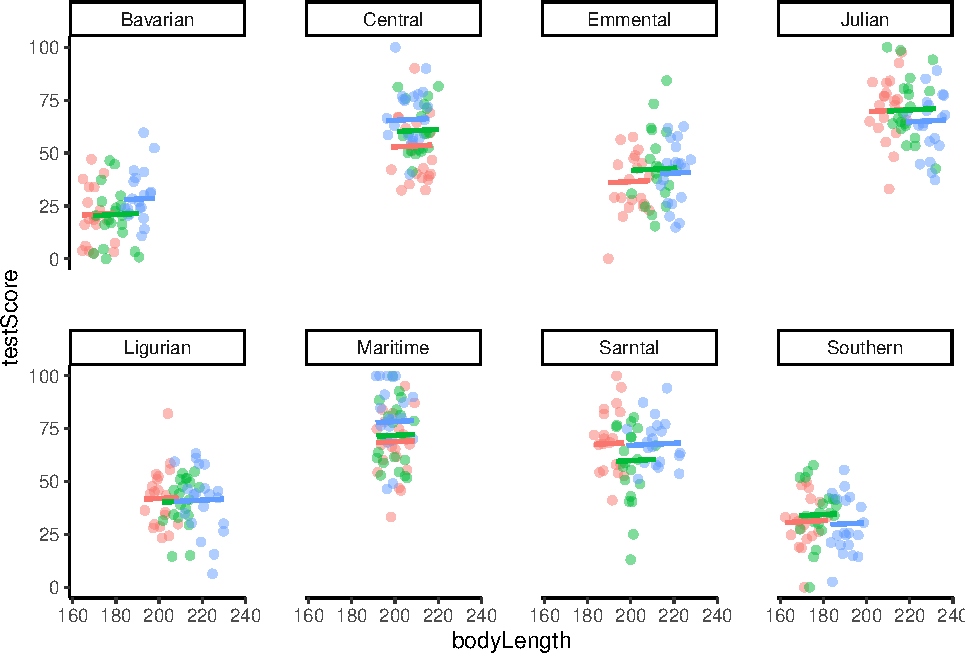
\includegraphics{Introduction-to-linear-mixed-models_files/figure-latex/unnamed-chunk-20-1.pdf}

\subsubsection{Introducing random
slopes}\label{introducing-random-slopes}

You might have noticed that all the lines on the above figure are
parallel: that's because so far, we have only fitted random-intercept
models. A random-intercept model allows the intercept to vary for each
level of the random effects, but keeps the slope constant among them. So
in our case, using this model means that we expect dragons in all
mountain ranges to exhibit the same relationship between body length and
intelligence (fixed slope), although we acknowledge that some
populations may be smarter or dumber to begin with (random intercept).

You can find an excellent visualisation of random intercepts and slopes
\href{https://mfviz.com/hierarchical-models/}{at this website}.

Now, in the life sciences, we perhaps more often assume that not all
populations would show the exact same relationship, for instance if your
study sites/populations are very far apart and have some relatively
important environmental, genetic, etc differences. Therefore, we often
want to fit a random-slope and random-intercept model. Maybe the dragons
in a very cold vs a very warm mountain range have evolved different body
forms for heat conservation and may therefore be smart even if they're
smaller than average.

We only need to make one change to our model to allow for random slopes
as well as intercept, and that's adding the fixed variable into the
random effect brackets:

\begin{Shaded}
\begin{Highlighting}[]
\NormalTok{mixed.ranslope }\OtherTok{\textless{}{-}} \FunctionTok{lmer}\NormalTok{(testScore }\SpecialCharTok{\textasciitilde{}}\NormalTok{ bodyLength2 }\SpecialCharTok{+}\NormalTok{ (}\DecValTok{1} \SpecialCharTok{+}\NormalTok{ bodyLength2}\SpecialCharTok{|}\NormalTok{mountainRange}\SpecialCharTok{/}\NormalTok{site), }\AttributeTok{data =}\NormalTok{ dragons)}
\end{Highlighting}
\end{Shaded}

\begin{verbatim}
## boundary (singular) fit: see help('isSingular')
\end{verbatim}

\begin{Shaded}
\begin{Highlighting}[]
\FunctionTok{summary}\NormalTok{(mixed.ranslope)}
\end{Highlighting}
\end{Shaded}

\begin{verbatim}
## Linear mixed model fit by REML ['lmerMod']
## Formula: testScore ~ bodyLength2 + (1 + bodyLength2 | mountainRange/site)
##    Data: dragons
## 
## REML criterion at convergence: 3968.4
## 
## Scaled residuals: 
##     Min      1Q  Median      3Q     Max 
## -3.2654 -0.6737 -0.0200  0.6931  2.8432 
## 
## Random effects:
##  Groups             Name        Variance Std.Dev. Corr 
##  site:mountainRange (Intercept)  19.8156  4.4515       
##                     bodyLength2   0.7178  0.8472  1.00 
##  mountainRange      (Intercept) 310.9691 17.6343       
##                     bodyLength2   6.1119  2.4722  -1.00
##  Residual                       208.5025 14.4396       
## Number of obs: 480, groups:  site:mountainRange, 24; mountainRange, 8
## 
## Fixed effects:
##             Estimate Std. Error t value
## (Intercept)  51.4263     6.3408   8.110
## bodyLength2   0.6691     1.8729   0.357
## 
## Correlation of Fixed Effects:
##             (Intr)
## bodyLength2 -0.461
## optimizer (nloptwrap) convergence code: 0 (OK)
## boundary (singular) fit: see help('isSingular')
\end{verbatim}

Here, we're saying, let's model the intelligence of dragons as a
function of body length, knowing that populations have different
intelligence baselines and that the relationship may vary among
populations.

Let's see that with a quick plot (we'll plot predictions in more detail
in the next section). Notice how the slopes for the different sites and
mountain ranges are not parallel anymore?

\begin{Shaded}
\begin{Highlighting}[]
\NormalTok{mixed.ranslope }\OtherTok{\textless{}{-}} \FunctionTok{lmer}\NormalTok{(testScore }\SpecialCharTok{\textasciitilde{}}\NormalTok{ bodyLength2 }\SpecialCharTok{+}\NormalTok{ (}\DecValTok{1} \SpecialCharTok{+}\NormalTok{ bodyLength2}\SpecialCharTok{|}\NormalTok{mountainRange}\SpecialCharTok{/}\NormalTok{site), }\AttributeTok{data =}\NormalTok{ dragons)}
\end{Highlighting}
\end{Shaded}

\begin{verbatim}
## boundary (singular) fit: see help('isSingular')
\end{verbatim}

\begin{Shaded}
\begin{Highlighting}[]
\FunctionTok{summary}\NormalTok{(mixed.ranslope)}
\end{Highlighting}
\end{Shaded}

\begin{verbatim}
## Linear mixed model fit by REML ['lmerMod']
## Formula: testScore ~ bodyLength2 + (1 + bodyLength2 | mountainRange/site)
##    Data: dragons
## 
## REML criterion at convergence: 3968.4
## 
## Scaled residuals: 
##     Min      1Q  Median      3Q     Max 
## -3.2654 -0.6737 -0.0200  0.6931  2.8432 
## 
## Random effects:
##  Groups             Name        Variance Std.Dev. Corr 
##  site:mountainRange (Intercept)  19.8156  4.4515       
##                     bodyLength2   0.7178  0.8472  1.00 
##  mountainRange      (Intercept) 310.9691 17.6343       
##                     bodyLength2   6.1119  2.4722  -1.00
##  Residual                       208.5025 14.4396       
## Number of obs: 480, groups:  site:mountainRange, 24; mountainRange, 8
## 
## Fixed effects:
##             Estimate Std. Error t value
## (Intercept)  51.4263     6.3408   8.110
## bodyLength2   0.6691     1.8729   0.357
## 
## Correlation of Fixed Effects:
##             (Intr)
## bodyLength2 -0.461
## optimizer (nloptwrap) convergence code: 0 (OK)
## boundary (singular) fit: see help('isSingular')
\end{verbatim}

Here, we're saying, let's model the intelligence of dragons as a
function of body length, knowing that populations have different
intelligence baselines and that the relationship may vary among
populations.

Let's see that with a quick plot (we'll plot predictions in more detail
in the next section). Notice how the slopes for the different sites and
mountain ranges are not parallel anymore?

\begin{Shaded}
\begin{Highlighting}[]
\NormalTok{mm\_plot }\OtherTok{\textless{}{-}} \FunctionTok{ggplot}\NormalTok{(dragons, }\FunctionTok{aes}\NormalTok{(}\AttributeTok{x =}\NormalTok{ bodyLength, }\AttributeTok{y =}\NormalTok{ testScore, }\AttributeTok{colour =}\NormalTok{ site))}\SpecialCharTok{+}
  \FunctionTok{facet\_wrap}\NormalTok{(}\SpecialCharTok{\textasciitilde{}}\NormalTok{mountainRange, }\AttributeTok{nrow =} \DecValTok{2}\NormalTok{)}\SpecialCharTok{+}
  \FunctionTok{geom\_point}\NormalTok{(}\AttributeTok{alpha =}\NormalTok{ .}\DecValTok{5}\NormalTok{)}\SpecialCharTok{+}
  \FunctionTok{theme\_classic}\NormalTok{()}\SpecialCharTok{+}
  \FunctionTok{geom\_line}\NormalTok{(}
    \AttributeTok{data =} \FunctionTok{cbind}\NormalTok{(dragons, }\AttributeTok{pred =} \FunctionTok{predict}\NormalTok{(mixed.ranslope)), }
    \FunctionTok{aes}\NormalTok{(}\AttributeTok{y =}\NormalTok{ pred), }
    \AttributeTok{linewidth =} \DecValTok{1}
\NormalTok{  )}\SpecialCharTok{+}
  \FunctionTok{theme}\NormalTok{(}
    \AttributeTok{legend.position =} \StringTok{\textquotesingle{}none\textquotesingle{}}\NormalTok{,}
    \AttributeTok{panel.spacing =} \FunctionTok{unit}\NormalTok{(}\DecValTok{2}\NormalTok{, }\StringTok{\textquotesingle{}lines\textquotesingle{}}\NormalTok{)}
\NormalTok{  )}
\NormalTok{mm\_plot}
\end{Highlighting}
\end{Shaded}

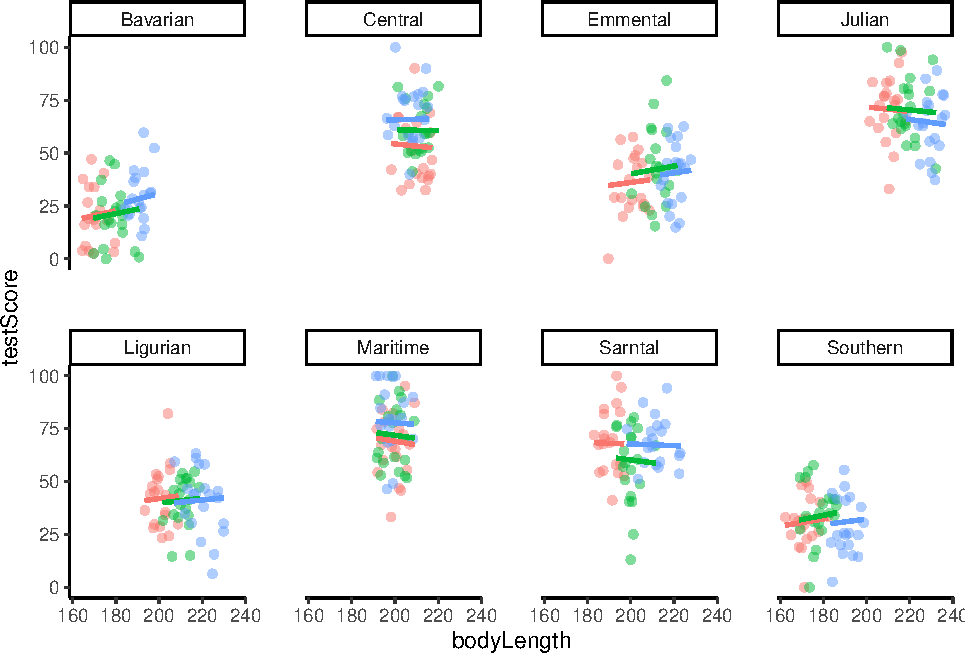
\includegraphics{Introduction-to-linear-mixed-models_files/figure-latex/unnamed-chunk-23-1.pdf}
Well done for getting here! You have now fitted random-intercept and
random-slopes, random-intercept mixed models and you know how to account
for hierarchical and crossed random effects. You saw that failing to
account for the correlation in data might lead to misleading results -
it seemed that body length affected the test score until we accounted
for the variation coming from mountain ranges. We can see now that body
length doesn't influence the test scores - great! We can pick smaller
dragons for any future training - smaller ones should be more
manageable!

If you are particularly keen, the next section gives you a few options
when it comes to presenting your model results and in the last ``extra''
section you can learn about the model selection conundrum. There is just
a little bit more code there to get through if you fancy those.

\subsection{Presenting your model
results}\label{presenting-your-model-results}

Once you get your model, you have to present it in a nicer form.

\subsubsection{Plotting model
predictions}\label{plotting-model-predictions}

Often you will want to visualise your model as a regression line with
some error around it, just like you would a simple linear model.
However, ggplot2 stats options are not designed to estimate mixed-effect
model objects correctly, so we will use the \texttt{ggeffects} package
to help us draw the plots.

\begin{Shaded}
\begin{Highlighting}[]
\CommentTok{\# Extract the prediction dataframe}
\NormalTok{pred.mm }\OtherTok{\textless{}{-}} \FunctionTok{ggpredict}\NormalTok{(mixed.lmer2, }\AttributeTok{terms =} \FunctionTok{c}\NormalTok{(}\StringTok{\textquotesingle{}bodyLength2\textquotesingle{}}\NormalTok{))}

\CommentTok{\# Plot the predictions}
\NormalTok{p }\OtherTok{\textless{}{-}} \FunctionTok{ggplot}\NormalTok{(pred.mm)}\SpecialCharTok{+}
  \FunctionTok{geom\_line}\NormalTok{(}\FunctionTok{aes}\NormalTok{(}\AttributeTok{x =}\NormalTok{ x, }\AttributeTok{y =}\NormalTok{ predicted))}\SpecialCharTok{+}   \CommentTok{\# slope}
  \FunctionTok{geom\_ribbon}\NormalTok{(}\FunctionTok{aes}\NormalTok{(}\AttributeTok{x =}\NormalTok{ x, }\AttributeTok{ymin =}\NormalTok{ predicted }\SpecialCharTok{{-}}\NormalTok{ std.error, }\AttributeTok{ymax =}\NormalTok{ predicted }\SpecialCharTok{+}\NormalTok{ std.error),}
              \AttributeTok{fill =} \StringTok{\textquotesingle{}lightgrey\textquotesingle{}}\NormalTok{, }\AttributeTok{alpha =}\NormalTok{ .}\DecValTok{5}\NormalTok{)}\SpecialCharTok{+}   \CommentTok{\# error band}
  \FunctionTok{geom\_point}\NormalTok{(}
    \AttributeTok{data =}\NormalTok{ dragons,}
    \FunctionTok{aes}\NormalTok{(}\AttributeTok{x =}\NormalTok{ bodyLength2, }\AttributeTok{y =}\NormalTok{ testScore, }\AttributeTok{colour =}\NormalTok{ mountainRange)}
\NormalTok{  )}\SpecialCharTok{+}
  \FunctionTok{labs}\NormalTok{(}
    \AttributeTok{x =} \StringTok{\textquotesingle{}Body Length (indexed)\textquotesingle{}}\NormalTok{, }\AttributeTok{y =} \StringTok{\textquotesingle{}Test score\textquotesingle{}}\NormalTok{,}
    \AttributeTok{title =} \StringTok{\textquotesingle{}Body length does not affect intelligence in dragons\textquotesingle{}}
\NormalTok{  )}\SpecialCharTok{+}
  \FunctionTok{theme\_minimal}\NormalTok{()}
\NormalTok{p}
\end{Highlighting}
\end{Shaded}

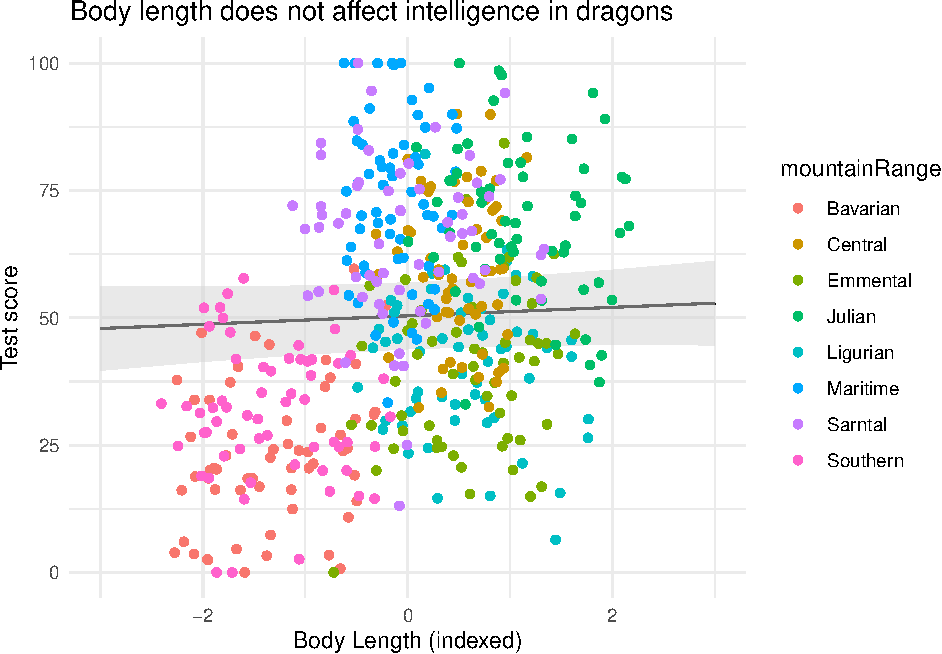
\includegraphics{Introduction-to-linear-mixed-models_files/figure-latex/unnamed-chunk-24-1.pdf}

What if you want to visualise how the relationships vary according to
different levels of random effects? You can specify
\texttt{type\ =\ "random"} (for ``random effects'') in the
\texttt{ggpredict()} function, and add the random effect name to the
\texttt{terms} argument.

\begin{Shaded}
\begin{Highlighting}[]
\CommentTok{\# Visualize one random effect {-}{-}{-}{-}}
\CommentTok{\# Extract the prediction dataframe}
\NormalTok{pred.mm2 }\OtherTok{\textless{}{-}} \FunctionTok{ggpredict}\NormalTok{(mixed.lmer2, }\AttributeTok{terms =} \FunctionTok{c}\NormalTok{(}\StringTok{\textquotesingle{}bodyLength2\textquotesingle{}}\NormalTok{, }\StringTok{\textquotesingle{}mountainRange\textquotesingle{}}\NormalTok{), }\AttributeTok{type =} \StringTok{\textquotesingle{}random\textquotesingle{}}\NormalTok{)}

\CommentTok{\# Check the structure of the ggeffects object:}
\FunctionTok{str}\NormalTok{(pred.mm2)}
\end{Highlighting}
\end{Shaded}

\begin{verbatim}
## Classes 'ggeffects' and 'data.frame':    56 obs. of  6 variables:
##  $ x        : num  -3 -3 -3 -3 -3 -3 -3 -3 -2 -2 ...
##  $ predicted: num  22.6 56.9 37.1 64.7 38.6 ...
##  $ std.error: num  8.23 8.23 8.23 8.23 8.23 ...
##  $ conf.low : num  6.4 40.7 20.9 48.5 22.4 ...
##  $ conf.high: num  38.8 73 53.3 80.9 54.8 ...
##  $ group    : Factor w/ 8 levels "Bavarian","Central",..: 1 2 3 4 5 6 7 8 1 2 ...
##  - attr(*, "legend.labels")= chr [1:8] "Bavarian" "Central" "Emmental" "Julian" ...
##  - attr(*, "x.is.factor")= chr "0"
##  - attr(*, "averaged_predictions")= logi FALSE
##  - attr(*, "continuous.group")= logi FALSE
##  - attr(*, "rawdata")='data.frame':  480 obs. of  6 variables:
##   ..$ response: num [1:480] 16.15 33.89 6.04 18.84 33.86 ...
##   ..$ x       : num [1:480] -2.21 -2.08 -2.19 -2.07 -1.93 ...
##   ..$ group   : Factor w/ 8 levels "Bavarian","Central",..: 1 1 1 1 1 1 1 1 1 1 ...
##   ..$ facet   : Factor w/ 1 level "1": 1 1 1 1 1 1 1 1 1 1 ...
##   ..$ panel   : Factor w/ 1 level "1": 1 1 1 1 1 1 1 1 1 1 ...
##   ..$ rowname : chr [1:480] "1" "2" "3" "4" ...
##  - attr(*, "title")= chr "Predicted values of testScore"
##  - attr(*, "x.title")= chr "bodyLength2"
##  - attr(*, "y.title")= chr "testScore"
##  - attr(*, "legend.title")= chr "mountainRange"
##  - attr(*, "constant.values")=List of 1
##   ..$ sample: chr "0 (population-level)"
##  - attr(*, "terms")= chr [1:2] "bodyLength2" "mountainRange"
##  - attr(*, "original.terms")= chr [1:2] "bodyLength2" "mountainRange"
##  - attr(*, "at.list")=List of 2
##   ..$ bodyLength2  : num [1:7] -3 -2 -1 0 1 2 3
##   ..$ mountainRange: chr [1:8] "Bavarian" "Central" "Emmental" "Julian" ...
##  - attr(*, "prediction.interval")= logi FALSE
##  - attr(*, "ci_level")= num 0.95
##  - attr(*, "type")= chr "random"
##  - attr(*, "response.name")= chr "testScore"
##  - attr(*, "back_transform")= logi TRUE
##  - attr(*, "response_transform")= chr "testScore"
##  - attr(*, "untransformed_predictions")= num [1:56] 22.6 56.9 37.1 64.7 38.6 ...
##  - attr(*, "standard_error")= num [1:56] 8.23 8.23 8.23 8.23 8.23 ...
##  - attr(*, "margin")= chr "mean_reference"
##  - attr(*, "df")= int 475
##  - attr(*, "family")= chr "gaussian"
##  - attr(*, "link")= chr "identity"
##  - attr(*, "logistic")= chr "0"
##  - attr(*, "is.trial")= chr "0"
##  - attr(*, "link_inverse")=function (eta)  
##  - attr(*, "link_function")=function (mu)  
##  - attr(*, "fitfun")= chr "lm"
##  - attr(*, "verbose")= logi TRUE
##  - attr(*, "model.name")= chr "mixed.lmer2"
\end{verbatim}

\begin{Shaded}
\begin{Highlighting}[]
\CommentTok{\# Plot the predictions}
\NormalTok{p }\OtherTok{\textless{}{-}} \FunctionTok{ggplot}\NormalTok{(pred.mm2)}\SpecialCharTok{+}
  \FunctionTok{geom\_line}\NormalTok{(}\FunctionTok{aes}\NormalTok{(}\AttributeTok{x =}\NormalTok{ x, }\AttributeTok{y =}\NormalTok{ predicted, }\AttributeTok{group =}\NormalTok{ group, }\AttributeTok{colour =}\NormalTok{ group))}\SpecialCharTok{+}   \CommentTok{\# slope}
  \FunctionTok{geom\_ribbon}\NormalTok{(}\FunctionTok{aes}\NormalTok{(}\AttributeTok{x =}\NormalTok{ x, }\AttributeTok{ymin =}\NormalTok{ predicted }\SpecialCharTok{{-}}\NormalTok{ std.error, }\AttributeTok{ymax =}\NormalTok{ predicted }\SpecialCharTok{+}\NormalTok{ std.error, }\AttributeTok{group =}\NormalTok{ group, }\AttributeTok{fill =}\NormalTok{ group), }\AttributeTok{alpha =}\NormalTok{ .}\DecValTok{15}\NormalTok{)}\SpecialCharTok{+}   \CommentTok{\# error band}
  \FunctionTok{geom\_point}\NormalTok{(}
    \AttributeTok{data =}\NormalTok{ dragons,}
    \FunctionTok{aes}\NormalTok{(}\AttributeTok{x =}\NormalTok{ bodyLength2, }\AttributeTok{y =}\NormalTok{ testScore, }\AttributeTok{colour =}\NormalTok{ mountainRange)}
\NormalTok{  )}\SpecialCharTok{+}
  \FunctionTok{labs}\NormalTok{(}
    \AttributeTok{x =} \StringTok{\textquotesingle{}Body Length (indexed)\textquotesingle{}}\NormalTok{, }\AttributeTok{y =} \StringTok{\textquotesingle{}Test score\textquotesingle{}}\NormalTok{,}
    \AttributeTok{title =} \StringTok{\textquotesingle{}Body length does not affect intelligence in dragons\textquotesingle{}}
\NormalTok{  )}\SpecialCharTok{+}
  \FunctionTok{theme\_minimal}\NormalTok{()}
\NormalTok{p}
\end{Highlighting}
\end{Shaded}

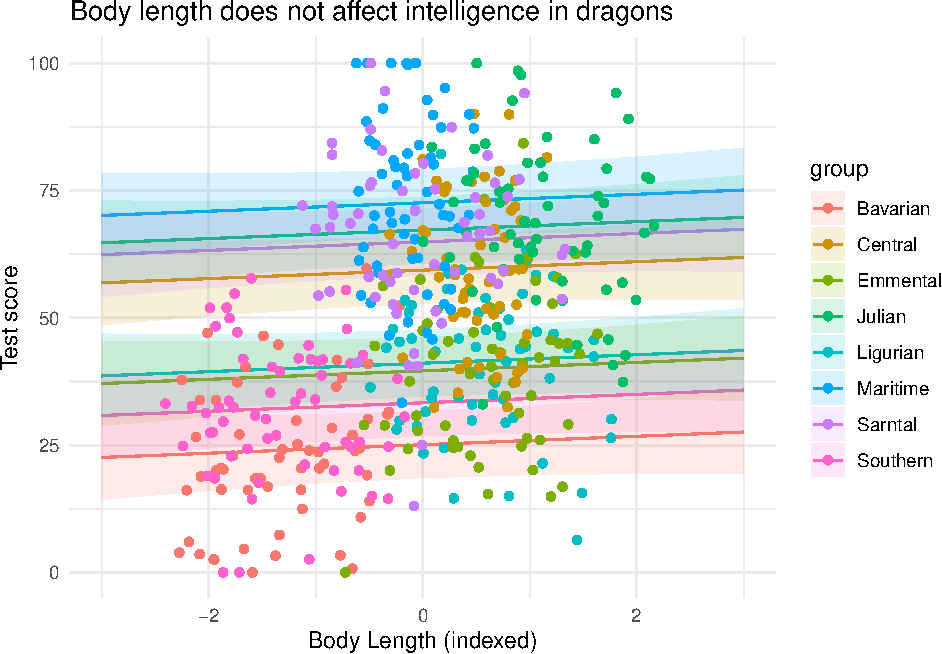
\includegraphics{Introduction-to-linear-mixed-models_files/figure-latex/unnamed-chunk-25-1.pdf}

\begin{Shaded}
\begin{Highlighting}[]
\CommentTok{\# Visualize both random effects {-}{-}{-}{-}}
\NormalTok{pred.mm3 }\OtherTok{\textless{}{-}} \FunctionTok{ggpredict}\NormalTok{(mixed.lmer2, }\AttributeTok{terms =} \FunctionTok{c}\NormalTok{(}\StringTok{\textquotesingle{}bodyLength2\textquotesingle{}}\NormalTok{, }\StringTok{\textquotesingle{}mountainRange\textquotesingle{}}\NormalTok{, }\StringTok{\textquotesingle{}sample\textquotesingle{}}\NormalTok{), }\AttributeTok{type =} \StringTok{\textquotesingle{}random\textquotesingle{}}\NormalTok{)}

\CommentTok{\# Check the structure of the ggeffects object:}
\FunctionTok{str}\NormalTok{(pred.mm3)}
\end{Highlighting}
\end{Shaded}

\begin{verbatim}
## Classes 'ggeffects' and 'data.frame':    1344 obs. of  7 variables:
##  $ x        : num  -3 -3 -3 -3 -3 -3 -3 -3 -3 -3 ...
##  $ predicted: num  20.1 19.5 26.3 16.2 23.4 ...
##  $ std.error: num  8.23 8.23 8.23 8.23 8.23 ...
##  $ conf.low : num  3.9359 3.3504 10.1388 0.0167 7.2485 ...
##  $ conf.high: num  36.3 35.7 42.5 32.4 39.6 ...
##  $ group    : Factor w/ 8 levels "Bavarian","Central",..: 1 1 1 1 1 1 1 1 1 1 ...
##  $ facet    : Factor w/ 24 levels "Bavarian:a","Bavarian:b",..: 1 2 3 4 5 6 7 8 9 10 ...
##  - attr(*, "legend.labels")= chr [1:8] "Bavarian" "Central" "Emmental" "Julian" ...
##  - attr(*, "x.is.factor")= chr "0"
##  - attr(*, "averaged_predictions")= logi FALSE
##  - attr(*, "continuous.group")= logi FALSE
##  - attr(*, "rawdata")='data.frame':  480 obs. of  6 variables:
##   ..$ response: num [1:480] 16.15 33.89 6.04 18.84 33.86 ...
##   ..$ x       : num [1:480] -2.21 -2.08 -2.19 -2.07 -1.93 ...
##   ..$ group   : Factor w/ 8 levels "Bavarian","Central",..: 1 1 1 1 1 1 1 1 1 1 ...
##   ..$ facet   : Factor w/ 24 levels "Bavarian:a","Bavarian:b",..: 1 1 1 1 1 1 1 1 1 1 ...
##   ..$ panel   : Factor w/ 1 level "1": 1 1 1 1 1 1 1 1 1 1 ...
##   ..$ rowname : chr [1:480] "1" "2" "3" "4" ...
##  - attr(*, "title")= chr "Predicted values of testScore"
##  - attr(*, "x.title")= chr "bodyLength2"
##  - attr(*, "y.title")= chr "testScore"
##  - attr(*, "legend.title")= chr "mountainRange"
##  - attr(*, "constant.values")= Named list()
##  - attr(*, "terms")= chr [1:3] "bodyLength2" "mountainRange" "sample"
##  - attr(*, "original.terms")= chr [1:3] "bodyLength2" "mountainRange" "sample"
##  - attr(*, "at.list")=List of 3
##   ..$ bodyLength2  : num [1:7] -3 -2 -1 0 1 2 3
##   ..$ mountainRange: chr [1:8] "Bavarian" "Central" "Emmental" "Julian" ...
##   ..$ sample       : chr [1:24] "Bavarian:a" "Bavarian:b" "Bavarian:c" "Central:a" ...
##  - attr(*, "prediction.interval")= logi FALSE
##  - attr(*, "ci_level")= num 0.95
##  - attr(*, "type")= chr "random"
##  - attr(*, "response.name")= chr "testScore"
##  - attr(*, "back_transform")= logi TRUE
##  - attr(*, "response_transform")= chr "testScore"
##  - attr(*, "untransformed_predictions")= num [1:1344] 20.1 19.5 26.3 16.2 23.4 ...
##  - attr(*, "standard_error")= num [1:1344] 8.23 8.23 8.23 8.23 8.23 ...
##  - attr(*, "margin")= chr "mean_reference"
##  - attr(*, "df")= int 475
##  - attr(*, "family")= chr "gaussian"
##  - attr(*, "link")= chr "identity"
##  - attr(*, "logistic")= chr "0"
##  - attr(*, "is.trial")= chr "0"
##  - attr(*, "link_inverse")=function (eta)  
##  - attr(*, "link_function")=function (mu)  
##  - attr(*, "fitfun")= chr "lm"
##  - attr(*, "verbose")= logi TRUE
##  - attr(*, "model.name")= chr "mixed.lmer2"
\end{verbatim}

\begin{Shaded}
\begin{Highlighting}[]
\CommentTok{\# Plot the predictions}
\NormalTok{p }\OtherTok{\textless{}{-}} \FunctionTok{ggplot}\NormalTok{(pred.mm3)}\SpecialCharTok{+}
  \FunctionTok{facet\_wrap}\NormalTok{(}\SpecialCharTok{\textasciitilde{}}\NormalTok{facet)}\SpecialCharTok{+}
  \FunctionTok{geom\_line}\NormalTok{(}\FunctionTok{aes}\NormalTok{(}\AttributeTok{x =}\NormalTok{ x, }\AttributeTok{y =}\NormalTok{ predicted, }\AttributeTok{group =}\NormalTok{ group, }\AttributeTok{colour =}\NormalTok{ group))}\SpecialCharTok{+}   \CommentTok{\# slope}
  \FunctionTok{geom\_ribbon}\NormalTok{(}\FunctionTok{aes}\NormalTok{(}\AttributeTok{x =}\NormalTok{ x, }\AttributeTok{ymin =}\NormalTok{ predicted }\SpecialCharTok{{-}}\NormalTok{ std.error, }\AttributeTok{ymax =}\NormalTok{ predicted }\SpecialCharTok{+}\NormalTok{ std.error, }\AttributeTok{group =}\NormalTok{ group, }\AttributeTok{fill =}\NormalTok{ group), }\AttributeTok{alpha =}\NormalTok{ .}\DecValTok{15}\NormalTok{)}\SpecialCharTok{+}   \CommentTok{\# error band}
  \FunctionTok{geom\_point}\NormalTok{(}
    \AttributeTok{data =}\NormalTok{ dragons,}
    \FunctionTok{aes}\NormalTok{(}\AttributeTok{x =}\NormalTok{ bodyLength2, }\AttributeTok{y =}\NormalTok{ testScore, }\AttributeTok{colour =}\NormalTok{ mountainRange)}
\NormalTok{  )}\SpecialCharTok{+}
  \FunctionTok{labs}\NormalTok{(}
    \AttributeTok{x =} \StringTok{\textquotesingle{}Body Length (indexed)\textquotesingle{}}\NormalTok{, }\AttributeTok{y =} \StringTok{\textquotesingle{}Test score\textquotesingle{}}\NormalTok{,}
    \AttributeTok{title =} \StringTok{\textquotesingle{}Body length does not affect intelligence in dragons\textquotesingle{}}
\NormalTok{  )}\SpecialCharTok{+}
  \FunctionTok{theme\_minimal}\NormalTok{()}
\NormalTok{p}
\end{Highlighting}
\end{Shaded}

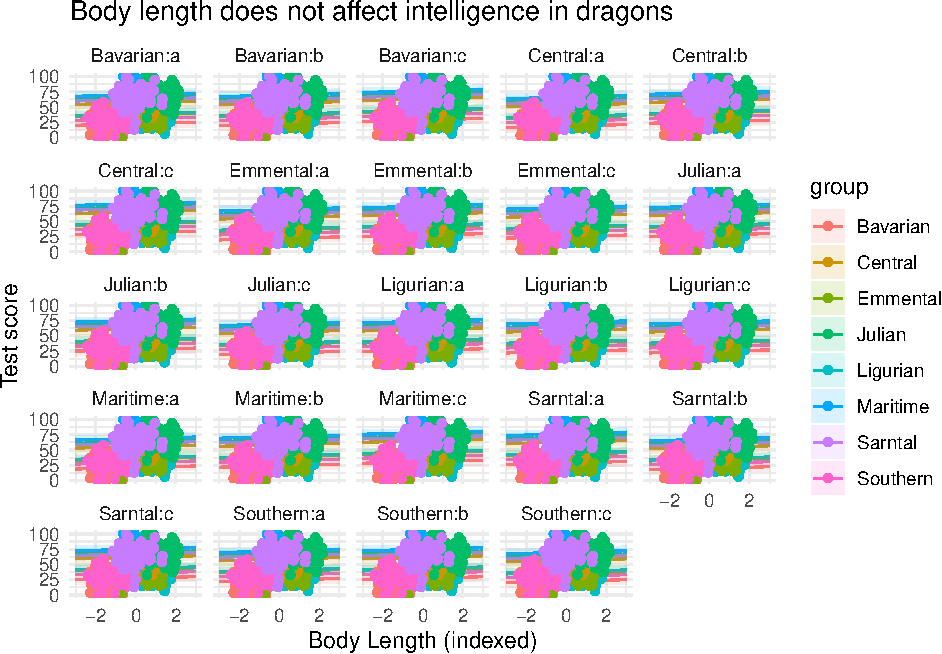
\includegraphics{Introduction-to-linear-mixed-models_files/figure-latex/unnamed-chunk-25-2.pdf}

We also demonstrate a way to plot the graph quicker with the
\texttt{plot()} function of ggEffects:

\begin{Shaded}
\begin{Highlighting}[]
\FunctionTok{ggpredict}\NormalTok{(mixed.lmer2, }\AttributeTok{terms =} \FunctionTok{c}\NormalTok{(}\StringTok{\textquotesingle{}bodyLength2\textquotesingle{}}\NormalTok{, }\StringTok{\textquotesingle{}mountainRange\textquotesingle{}}\NormalTok{), }\AttributeTok{type =} \StringTok{\textquotesingle{}random\textquotesingle{}}\NormalTok{) }\SpecialCharTok{\%\textgreater{}\%} 
  \FunctionTok{plot}\NormalTok{()}\SpecialCharTok{+}
  \FunctionTok{labs}\NormalTok{(}
    \AttributeTok{x =} \StringTok{\textquotesingle{}Body Length\textquotesingle{}}\NormalTok{,}
    \AttributeTok{y =} \StringTok{\textquotesingle{}Test Score\textquotesingle{}}\NormalTok{,}
    \AttributeTok{title =} \StringTok{\textquotesingle{}Effect of body size on intelligence of dragons\textquotesingle{}}
\NormalTok{  )}\SpecialCharTok{+}
  \FunctionTok{theme\_minimal}\NormalTok{()}
\end{Highlighting}
\end{Shaded}

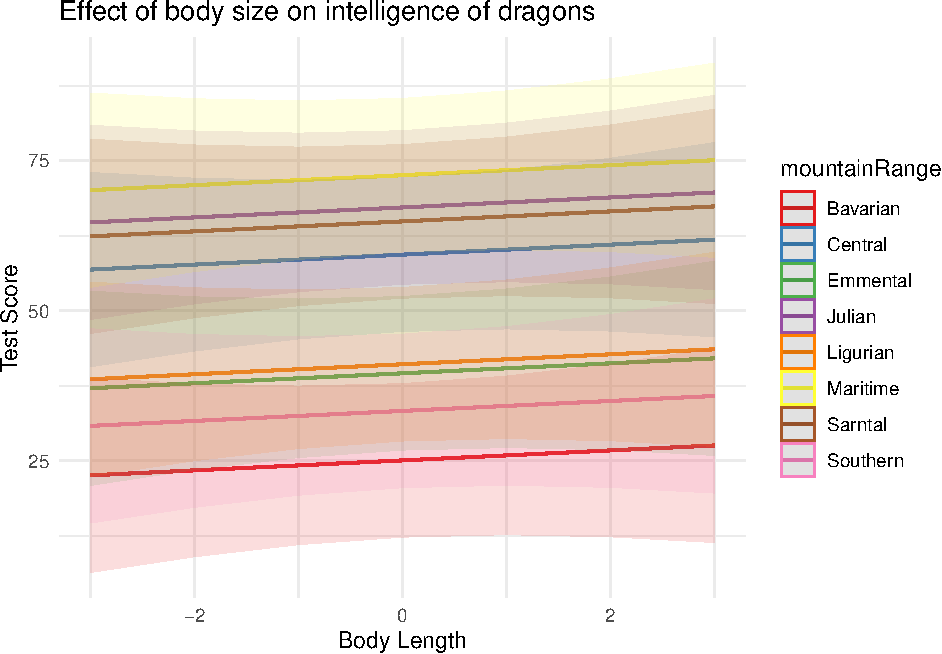
\includegraphics{Introduction-to-linear-mixed-models_files/figure-latex/unnamed-chunk-26-1.pdf}

You can clearly see the random intercepts and fixed slopes from this
graph. When assessing the quality of your model, it's always a good idea
to look at the raw data, the summary output, and the predictions all
together to make sure you understand what is going on (and that you have
specified the model correctly).

Another way to visualise mixed model results, if you are interested in
showing the variation among levels of your random effects, is to plot
the departure from the overall model estimate for intercepts - and
slopes, if you have a random slope model:

\begin{Shaded}
\begin{Highlighting}[]
\CommentTok{\# Visualize random effects}
\NormalTok{(re.effects }\OtherTok{\textless{}{-}} \FunctionTok{plot\_model}\NormalTok{(mixed.ranslope, }\AttributeTok{type =} \StringTok{\textquotesingle{}re\textquotesingle{}}\NormalTok{, }\AttributeTok{show.values =} \ConstantTok{TRUE}\NormalTok{))}
\end{Highlighting}
\end{Shaded}

\begin{verbatim}
## [[1]]
\end{verbatim}

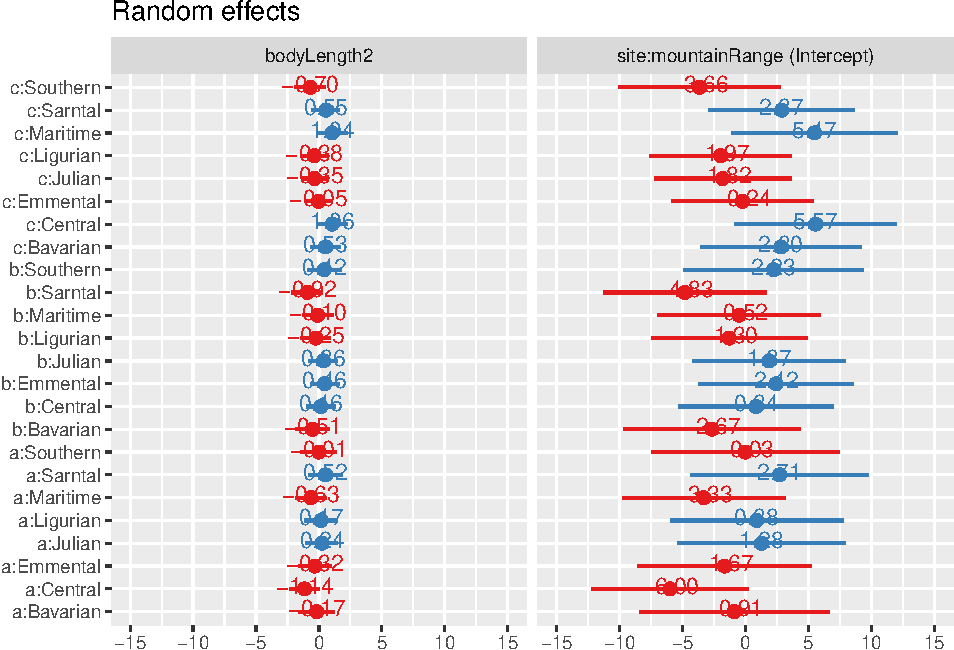
\includegraphics{Introduction-to-linear-mixed-models_files/figure-latex/unnamed-chunk-27-1.pdf}

\begin{verbatim}
## 
## [[2]]
\end{verbatim}

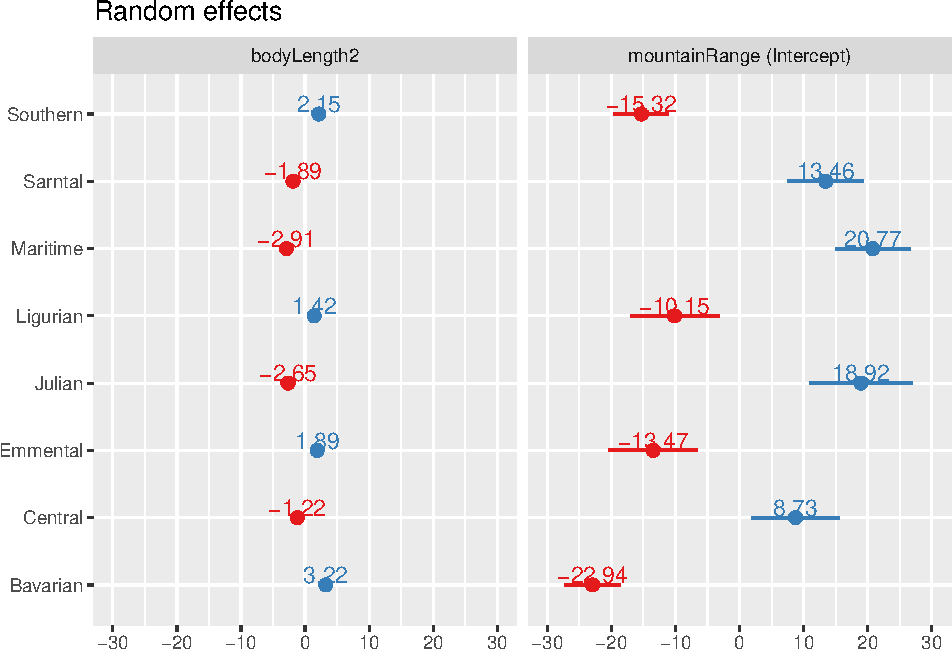
\includegraphics{Introduction-to-linear-mixed-models_files/figure-latex/unnamed-chunk-27-2.pdf}

\begin{Shaded}
\begin{Highlighting}[]
\CommentTok{\# Show summary}
\FunctionTok{summary}\NormalTok{(mixed.ranslope)}
\end{Highlighting}
\end{Shaded}

\begin{verbatim}
## Linear mixed model fit by REML ['lmerMod']
## Formula: testScore ~ bodyLength2 + (1 + bodyLength2 | mountainRange/site)
##    Data: dragons
## 
## REML criterion at convergence: 3968.4
## 
## Scaled residuals: 
##     Min      1Q  Median      3Q     Max 
## -3.2654 -0.6737 -0.0200  0.6931  2.8432 
## 
## Random effects:
##  Groups             Name        Variance Std.Dev. Corr 
##  site:mountainRange (Intercept)  19.8156  4.4515       
##                     bodyLength2   0.7178  0.8472  1.00 
##  mountainRange      (Intercept) 310.9691 17.6343       
##                     bodyLength2   6.1119  2.4722  -1.00
##  Residual                       208.5025 14.4396       
## Number of obs: 480, groups:  site:mountainRange, 24; mountainRange, 8
## 
## Fixed effects:
##             Estimate Std. Error t value
## (Intercept)  51.4263     6.3408   8.110
## bodyLength2   0.6691     1.8729   0.357
## 
## Correlation of Fixed Effects:
##             (Intr)
## bodyLength2 -0.461
## optimizer (nloptwrap) convergence code: 0 (OK)
## boundary (singular) fit: see help('isSingular')
\end{verbatim}

Careful here! The values you see are NOT actual values, but rather the
difference between the general intercept or slope value found in your
model summary and the estimate for this specific level of random effect.
For instance, the relationship for dragons in the Maritime mountain
range would have a slope of (-2.91 + 0.67) = -2.24 and an intercept of
(20.77 + 51.43) = 72.20.

If you are looking for more ways to create plots of your results, check
out \texttt{dotwhisker} and
\href{https://cran.r-project.org/web/packages/dotwhisker/vignettes/dotwhisker-vignette.html}{this
tutorial}.

\subsubsection{Tables}\label{tables}

For lme4, if you are looking for a table, I'd recommend that you have a
look at the \texttt{stargazer} package.

\texttt{stargazeris} very nicely annotated and there are lots of
resources
(e.g.~\href{https://cran.r-project.org/web/packages/stargazer/vignettes/stargazer.pdf}{this})
out there and a
\href{http://jakeruss.com/cheatsheets/stargazer.html}{great cheat sheet}
so I won't go into too much detail, as I'm confident you will find
everything you need.

Here is a quick example - simply plug in your model name, in this case
mixed.lmer2 into the stargazer function. I set type to ``text'' so that
you can see the table in your console. I usually tweak the table like
this until I'm happy with it and then export it using type = ``latex'',
but ``html'' might be more useful for you if you are not a LaTeX user.

If you are keen, explore this table a little further - what would you
change? What would you get rid off?

\begin{Shaded}
\begin{Highlighting}[]
\CommentTok{\# Plain text table}
\FunctionTok{stargazer}\NormalTok{(}
\NormalTok{  mixed.lmer2,}
  \AttributeTok{type =} \StringTok{\textquotesingle{}text\textquotesingle{}}\NormalTok{,}
  \AttributeTok{digits =} \DecValTok{3}\NormalTok{,}
  \AttributeTok{star.cutoffs =} \FunctionTok{c}\NormalTok{(.}\DecValTok{05}\NormalTok{, .}\DecValTok{01}\NormalTok{, .}\DecValTok{001}\NormalTok{),}
  \AttributeTok{digit.separator =} \StringTok{\textquotesingle{}\textquotesingle{}}
\NormalTok{)}
\end{Highlighting}
\end{Shaded}

\begin{verbatim}
## 
## =================================================
##                          Dependent variable:     
##                     -----------------------------
##                               testScore          
## -------------------------------------------------
## bodyLength2                     0.831            
##                                (1.681)           
##                                                  
## Constant                      50.386***          
##                                (6.507)           
##                                                  
## -------------------------------------------------
## Observations                     480             
## Log Likelihood                -1985.195          
## Akaike Inf. Crit.             3980.389           
## Bayesian Inf. Crit.           4001.258           
## =================================================
## Note:               *p<0.05; **p<0.01; ***p<0.001
\end{verbatim}

\subsubsection{Tables (a better way)}\label{tables-a-better-way}

Using the \texttt{modelsummary} package is recommended nowadays. It can
automatically detect whether the output of the document should be HTML,
PDF, or anything else. Highly recommended over \texttt{stargazer}.

\paragraph{modelsummary}\label{modelsummary}

\begin{Shaded}
\begin{Highlighting}[]
\CommentTok{\# Generate the table}
\FunctionTok{modelsummary}\NormalTok{(}
  \FunctionTok{list}\NormalTok{(}\StringTok{"Mixed Model"} \OtherTok{=}\NormalTok{ mixed.lmer2),}
  \AttributeTok{fmt =} \DecValTok{3}\NormalTok{,                             }\CommentTok{\# Default number format for estimates}
  \AttributeTok{stars =} \FunctionTok{c}\NormalTok{(}\StringTok{\textquotesingle{}*\textquotesingle{}} \OtherTok{=} \FloatTok{0.05}\NormalTok{, }\StringTok{\textquotesingle{}**\textquotesingle{}} \OtherTok{=} \FloatTok{0.01}\NormalTok{, }\StringTok{\textquotesingle{}***\textquotesingle{}} \OtherTok{=} \FloatTok{0.001}\NormalTok{), }\CommentTok{\# Define stars}
  \AttributeTok{title =} \StringTok{"Model Summary using modelsummary"}\NormalTok{,}
  \AttributeTok{notes =} \FunctionTok{list}\NormalTok{(}\StringTok{"Standard errors in parentheses."}\NormalTok{,}
               \StringTok{"Signif. codes: * p\textless{}0.05; ** p\textless{}0.01; *** p\textless{}0.001"}\NormalTok{) }\CommentTok{\# Add notes}
\NormalTok{)}
\end{Highlighting}
\end{Shaded}

\begin{table}
\centering
\begin{talltblr}[         %% tabularray outer open
caption={Model Summary using modelsummary},
note{}={* p \num{< 0.05}, ** p \num{< 0.01}, *** p \num{< 0.001}},
note{ }={Standard errors in parentheses.},
note{  }={Signif. codes: * p<0.05; ** p<0.01; *** p<0.001},
]                     %% tabularray outer close
{                     %% tabularray inner open
colspec={Q[]Q[]},
column{2}={}{halign=c,},
column{1}={}{halign=l,},
hline{9}={1,2}{solid, black, 0.05em},
}                     %% tabularray inner close
\toprule
& Mixed Model \\ \midrule %% TinyTableHeader
(Intercept) & \num{50.386}*** \\
& (\num{6.507}) \\
bodyLength2 & \num{0.831} \\
& (\num{1.681}) \\
SD (Intercept sample) & \num{4.805} \\
SD (Intercept mountainRange) & \num{18.099} \\
SD (Observations) & \num{14.442} \\
Num.Obs. & \num{480} \\
R2 Marg. & \num{0.001} \\
R2 Cond. & \num{0.627} \\
AIC & \num{3980.4} \\
BIC & \num{4001.3} \\
ICC & \num{0.6} \\
RMSE & \num{14.14} \\
\bottomrule
\end{talltblr}
\end{table}

\subsubsection{Further processing}\label{further-processing}

If you'd like to be able to do more with your model results, for
instance process them further, collate model results from multiple
models or plot, them have a look at the \texttt{broom} package. This
\href{http://varianceexplained.org/r/broom-intro/}{tutorial} is a great
start.

\subsection{EXTRA: P-values and model
selection}\label{extra-p-values-and-model-selection}

Please be very, very careful when it comes to model selection. Focus on
your question, don't just plug in and drop variables from a model
haphazardly until you make something ``significant''. Always choose
variables based on biology/ecology: I might use model selection to check
a couple of non-focal parameters, but I keep the ``core'' of the model
untouched in most cases. Define your goals and questions and focus on
that. Also, don't just put all possible variables in (i.e.~don't
overfit). Remember that as a rule of thumb, you need 10 times more data
than parameters you are trying to estimate.

For more info on overfitting check out this
\href{https://ourcodingclub.github.io/tutorials/modelling/}{tutorial}.

\subsubsection{Fixed effects structure}\label{fixed-effects-structure}

Before we start, again: think twice before trusting model selection!

Most of you are probably going to be predominantly interested in your
fixed effects, so let's start here. lme4 doesn't spit out p-values for
the parameters by default. This is a conscious choice made by the
authors of the package, as there are many problems with p-values (I'm
sure you are aware of the debates!).

You will inevitably look for a way to assess your model though so here
are a few solutions on how to go about hypothesis testing in linear
mixed models (LMMs):

From worst to best:

\begin{itemize}
\tightlist
\item
  Wald Z-tests
\item
  Wald t-tests (but LMMs need to be balanced and nested)
\item
  Likelihood ratio tests (via anova() or drop1())
\item
  MCMC or parametric bootstrap confidence intervals
\end{itemize}

See
\href{http://stats.stackexchange.com/questions/95054/how-to-get-an-overall-p-value-and-effect-size-for-a-categorical-factor-in-a-mi}{this
link} for more information and further reading.

I think that MCMC and bootstrapping are a bit out of our reach for this
workshop so let's have a quick go at \textbf{likelihood ratio tests}
using \texttt{anova()}. With large sample sizes, p-values based on the
likelihood ratio are generally considered okay. \textbf{NOTE}: With
small sample sizes, you might want to look into deriving p-values using
the Kenward-Roger or Satterthwaite approximations (for REML models).
Check out the \texttt{pbkrtest} package.

Fit the models, a full model and a reduced model in which we dropped our
fixed effect (\texttt{bodyLength2}):

\begin{Shaded}
\begin{Highlighting}[]
\NormalTok{full.lmer }\OtherTok{\textless{}{-}} \FunctionTok{lmer}\NormalTok{(testScore }\SpecialCharTok{\textasciitilde{}}\NormalTok{ bodyLength2 }\SpecialCharTok{+}\NormalTok{ (}\DecValTok{1}\SpecialCharTok{|}\NormalTok{mountainRange) }\SpecialCharTok{+}\NormalTok{ (}\DecValTok{1}\SpecialCharTok{|}\NormalTok{sample), }
                  \AttributeTok{data =}\NormalTok{ dragons, }\AttributeTok{REML =} \ConstantTok{FALSE}\NormalTok{)}
\NormalTok{reduced.lmer }\OtherTok{\textless{}{-}} \FunctionTok{lmer}\NormalTok{(testScore }\SpecialCharTok{\textasciitilde{}} \DecValTok{1} \SpecialCharTok{+}\NormalTok{ (}\DecValTok{1}\SpecialCharTok{|}\NormalTok{mountainRange) }\SpecialCharTok{+}\NormalTok{ (}\DecValTok{1}\SpecialCharTok{|}\NormalTok{sample), }
                         \AttributeTok{data =}\NormalTok{ dragons, }\AttributeTok{REML =} \ConstantTok{FALSE}\NormalTok{)}
\end{Highlighting}
\end{Shaded}

Compare them:

\begin{Shaded}
\begin{Highlighting}[]
\FunctionTok{anova}\NormalTok{(reduced.lmer, full.lmer)}
\end{Highlighting}
\end{Shaded}

\begin{verbatim}
## Data: dragons
## Models:
## reduced.lmer: testScore ~ 1 + (1 | mountainRange) + (1 | sample)
## full.lmer: testScore ~ bodyLength2 + (1 | mountainRange) + (1 | sample)
##              npar    AIC    BIC  logLik -2*log(L)  Chisq Df Pr(>Chisq)
## reduced.lmer    4 3987.1 4003.7 -1989.5    3979.1                     
## full.lmer       5 3988.8 4009.6 -1989.4    3978.8 0.2868  1     0.5923
\end{verbatim}

Notice that we have fitted our models with \texttt{REML\ =\ FALSE}.

\textbf{REML} stands for \textbf{restricted (or ``residual'') maximum
likelihood} and it is the default parameter estimation criterion for
linear mixed models. As you probably guessed, \textbf{ML} stands for
\textbf{maximum likelihood} - you can set \texttt{REML\ =\ FALSE} in
your call to lmer to use ML estimates. However, \textbf{ML estimates are
known to be biased} and with REML being usually less biased,
\textbf{REML estimates of variance components are generally preferred}.
This is why in our previous models we skipped setting REML - we just
left it as default (i.e.~\texttt{REML\ =\ TRUE}).

\textbf{REML} assumes that the fixed effects structure is correct. You
\textbf{should use maximum likelihood when comparing models with
different fixed effects}, as \textbf{ML} doesn't rely on the
coefficients of the fixed effects - and that's why we are refitting our
full and reduced models above with the addition of
\texttt{REML\ =\ FALSE} in the call.

\textbf{NOTE 1}: Even though you use \textbf{ML to compare models}, you
should \textbf{report parameter estimates from your final ``best'' REML
model}, as ML may underestimate variance of the random effects.

\textbf{NOTE 2}: Models can also be compared using the \textbf{AICc}
function from the \textbf{AICcmodavg} package. The Akaike Information
Criterion (AIC) is a measure of model quality. AICc corrects for bias
created by small sample size when estimating AIC. Generally, if models
are within 2 AICc units of each other they are very similar. Within 5
units they are quite similar, over 10 units difference and you can
probably be happy with the model with lower AICc. As with p-values
though, there is no ``hard line'' that's always correct.

\textbf{NOTE 3}: There isn't really an agreed upon way of dealing with
the variance from the random effects in mixed models when it comes to
assessing significance. Both \textbf{p-values} and \textbf{effect sizes}
have issues, although from what I gather, \textbf{p-values} seem to
cause more disagreement than \textbf{effect sizes}, at least in the R
community.

\subsubsection{Random effects structure}\label{random-effects-structure}

Now you might wonder about selecting your random effects. In general,
I'd advise you to think about your \textbf{experimental design, your
system and data collected, as well as your questions}.

If your random effects are there to deal with
\textbf{pseudoreplication}, then it doesn't really matter whether they
are ``significant'' or not: they \textbf{are part of your design} and
have to be included. Imagine we tested our dragons multiple times - we
then have to fit dragon identity as a random effect.

On the other hand, if you are trying to account for other variability
that you think might be important, it becomes a bit harder. Imagine we
measured the mass of our dragons over their lifespans (let's say 100
years). We might then want to fit year as a random effect to account for
any temporal variation - maybe some years were affected by drought, the
resources were scarce and so dragon mass was negatively impacted. Year
would definitely be a sensible random effect, although strictly speaking
not a must.

When it comes to such random effects you can use \textbf{model
selection} to help you decide what to keep in. Following Zuur's advice,
we \textbf{use \texttt{REML} estimators for comparison of models with
different random effects} (we keep fixed effects constant). (Zuur: ``Two
models with nested random structures cannot be done with ML because the
estimators for the variance terms are biased.'' )

\textbf{NOTE 1}: Do \textbf{NOT} vary random and fixed effects at the
same time - either deal with your random effects structure or with your
fixed effects structure at any given point.

\textbf{NOTE 2}: Do \textbf{NOT} compare \texttt{lmer} models with
\texttt{lm} models (or \texttt{glmer} with \texttt{glm}).

\subsubsection{Entire model selection}\label{entire-model-selection}

A few notes on the process of model selection. There are two ways here:
(i) \textbf{``top-down''}, where you start with a complex model and
gradually reduce it, and (ii) \textbf{``step up''}, where you start with
a simple model and add new variables to it. Unfortunately, you might
arrive at different final models by using those strategies and so you
need to be careful.

The model selection process recommended by Zuur et al.~(2009) is a
top-down strategy and goes as follows:

\begin{enumerate}
\def\labelenumi{\arabic{enumi}.}
\tightlist
\item
  fit a \textbf{full model} (he even recommends ``beyond optimal''
  i.e.~more complex than you'd expect or want it to be)
\item
  sort out the \textbf{random effects structure} (use \texttt{REML}
  likelihoods or \texttt{REML} AIC or BIC)
\item
  sort out \textbf{fixed effects structure} (either use \texttt{REML}
  the F-statistic or the t-statistic or compare nested \texttt{ML}
  models - keep your random effects constant)
\item
  once you arrive at the \textbf{final model present it using
  \texttt{REML} estimation}
\end{enumerate}

\textbf{NOTE}: At the risk of sounding like a broken record: I think
it's best to decide on what your model is based on biology/ecology/data
structure etc. than through following model selection blindly.
Additionally, just because something is non-significant doesn't
necessarily mean you should always get rid of it.

\subsection{THE END}\label{the-end}

\textbf{Well done for getting through this!} As you probably gather,
mixed effects models can be a bit tricky and often there isn't much
consensus on the best way to tackle something within them. The coding
bit is actually the (relatively) easy part here. Be mindful of what you
are doing, prepare the data well and things should be alright.

Keen to take your modelling skills to the next level? If you want to
learn hierarchical spatial modelling and accounting for spatial
autocorrelation, \textbf{check out our tutorial on INLA}!

\end{document}
